\section{Adaptation of LLMs}
\label{sec-adaptation}

After pre-training, LLMs can acquire the general abilities for  solving various tasks. However, an increasing number of studies have shown  that LLM's abilities can be further adapted according to specific goals.
In this section, we introduce two major approaches to adapting pre-trained LLMs, namely instruction tuning and alignment tuning. The former approach  mainly aims to enhance (or unlock) the abilities of LLMs, while the latter approach aims to align the behaviors of LLMs with human values or preferences. 
Further, we will also discuss  efficient tuning and quantization for  model adaptation in resource-limited settings.  
In what follows, we will introduce the four parts in detail. 

\begin{figure*}[h]
    \centering
    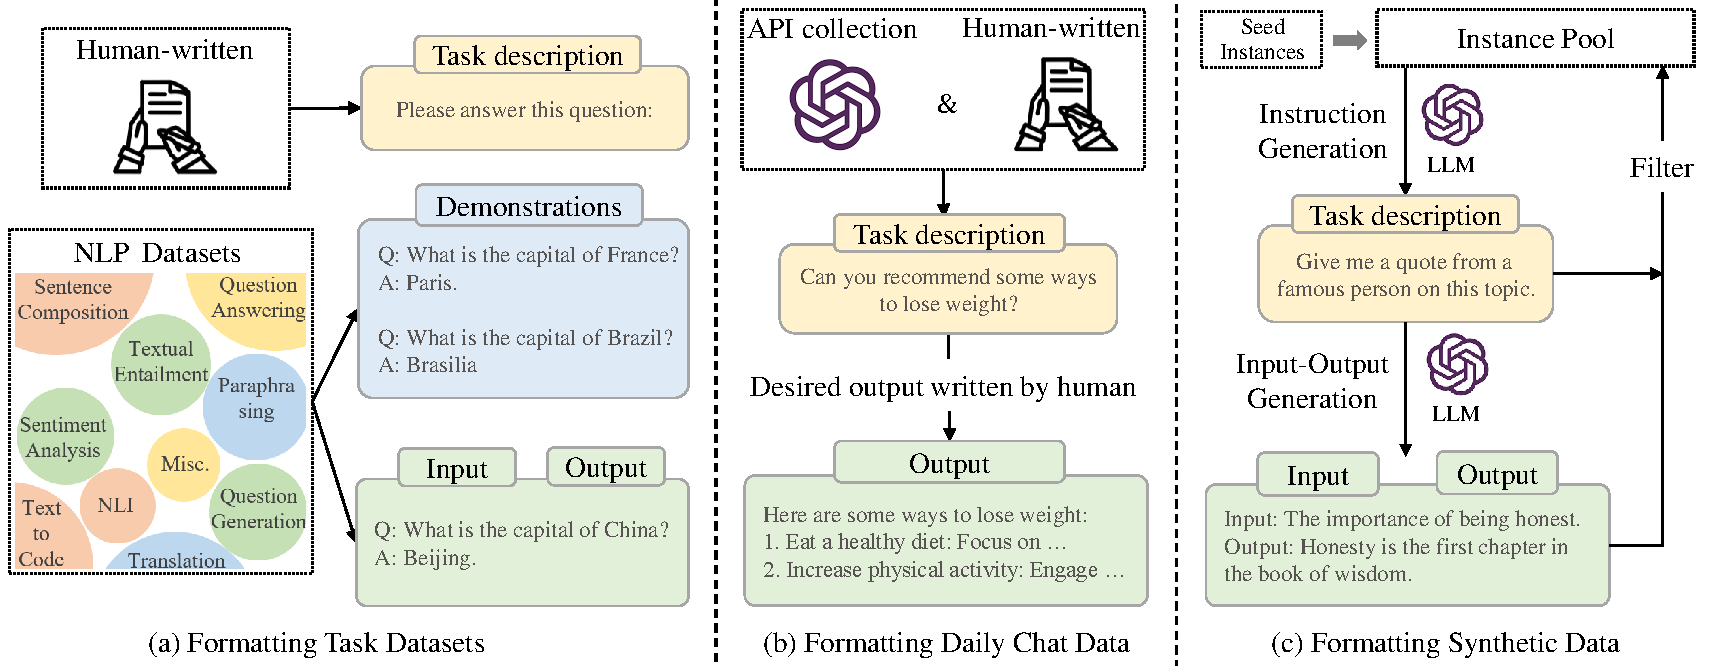
\includegraphics[width=1\textwidth]{images/Instruction-Tuning-new.pdf}
    \caption{An illustration of instance formatting and three different methods for constructing the instruction-formatted instances. }
    \label{fig:instruction-tuning}
\end{figure*}



\subsection{Instruction Tuning}
\label{sec-instruction}
In essence, instruction tuning is the approach to fine-tuning  pre-trained  LLMs on a collection of formatted instances in the form of natural language~\cite{Wei-ICLR-2022-Finetuned}, which is highly related to supervised fine-tuning~\cite{Ouyang-arxiv-2022-Training} and multi-task prompted training~\cite{Sanh-ICLR-2022-Multitask}. %
In order to perform instruction tuning, we first need to collect or construct instruction-formatted instances. 
Then, we employ these formatted instances to fine-tune LLMs in a supervised learning way (\eg training with the sequence-to-sequence loss). 
After instruction tuning, LLMs can demonstrate superior abilities to generalize to unseen tasks~\cite{Wei-ICLR-2022-Finetuned,Sanh-ICLR-2022-Multitask,Chung-arxiv-2022-Scaling}, even in a multilingual setting~\cite{Muennighoff-2022-arxiv-Crosslingual}. 


A recent survey~\cite{Lou-arXiv-2023-Is} presents a systematic overview of the research on instruction tuning. In comparison to that, we mainly focus on the effect of instruction tuning on LLMs and provide detailed guidelines or strategies for instance collection and tuning. In addition, we also discuss the use of instruction tuning for satisfying the real needs of users, which has been widely applied in existing LLMs, \eg InstructGPT~\cite{Ouyang-arxiv-2022-Training} and GPT-4~\cite{OpenAI-OpenAI-2023-GPT-4}.



\subsubsection{Formatted Instance Construction}\label{sec-instruction-formatted} 
Generally, an instruction-formatted instance consists of a task description (called an \emph{instruction}), an optional input, the corresponding output, and a small number of demonstrations (optional).
As important public resources, existing studies have released a large number of labeled data formatted in natural language (see the list of available resources in Table~\ref{tab:instruction-collection}) as introduced in Section~\ref{sec:it-dataset}. 
Next, we introduce three major methods for constructing formatted instances (see an illustration in Figure~\ref{fig:instruction-tuning}) and then discuss several key factors for instance construction.  



\paratitle{Formatting NLP Task Datasets.} 
Before instruction tuning was proposed, several early  studies~\cite{Liu-ACL-2019-Multi,Aghajanyan-EMNLP-2021-Muppet,Tang-arxiv-2022-MVP} collected the instances from a diverse range of traditional NLP tasks (\eg text summarization, text classification, and translation) to create supervised multi-task training datasets. 
As a major source of instruction tuning instances, it is convenient to format these multi-task training  datasets with natural language task descriptions. 
Specifically, recent work~\cite{Wei-ICLR-2022-Finetuned,Sanh-ICLR-2022-Multitask,Ouyang-arxiv-2022-Training,Wang-EMNLP-2022-Super}  augments the labeled datasets with human-written task descriptions, which instructs LLMs to understand the tasks by explaining the task goal.  %
For example, in Figure~\ref{fig:instruction-tuning}(a),  a task description ``\emph{Please answer this question}'' is added for each example in the question-answering task. 
After instruction tuning, LLMs can generalize well to other unseen tasks by following their task descriptions~\cite{Wei-ICLR-2022-Finetuned,Sanh-ICLR-2022-Multitask,Chung-arxiv-2022-Scaling}. 
In particular, it has been shown that instructions are the crucial factor in task generalization ability for LLMs~\cite{Wei-ICLR-2022-Finetuned}:  
by fine-tuning the model on labeled datasets with the task descriptions removed, it results in a dramatic drop in model performance.
To better generate labeled instances for instruction tuning, a crowd-sourcing platform, PromptSource~\cite{Bach-ACL-2022-PromptSource} has been proposed to effectively create, share, and verify the task descriptions for different datasets.  
To enrich the training instances, several studies~\cite{Sanh-ICLR-2022-Multitask,Tang-arxiv-2022-MVP,Longpre-arxiv-2023-The} also try to invert the input-output pairs of existing instances with specially designed task descriptions for instruction tuning. For instance, given a question-answer pair, we can create a new instance by predicting the answer-conditioned question (\eg \emph{``Please generate a question based on the answer:''}). %

\paratitle{Formatting Daily Chat Data.}
Despite that a large number of training instances have been formatted with instructions, they mainly come from public NLP datasets, either lacking instruction diversity or mismatching with real human needs~\cite{Ouyang-arxiv-2022-Training}.   
To overcome this issue, InstructGPT~\cite{Ouyang-arxiv-2022-Training} proposes to take the queries that real users have submitted to the OpenAI API as the task descriptions.  %
Additionally, to enrich the task diversity, human labelers are also asked to compose the instructions for real-life tasks, including open-ended generation, open question answering, brainstorming, and chatting. 
Then, they let another group of labelers directly answer these instructions as the output.
Finally, they pair one instruction (\ie the collected user query) and the expected output  (\ie the human-written answer) as a training instance.
Note that InstructGPT also employs these real-world tasks formatted in natural language for alignment tuning (discussed in Section~\ref{sec-alignment}). 
Further, GPT-4~\cite{OpenAI-OpenAI-2023-GPT-4} has designed potentially high-risk instructions and guided the model to reject these instructions through supervised fine-tuning for safety concerns. 
{Considering the absence of high-quality public chat data, several studies have also collected  users' chat requests as input data,  and then utilized ChatGPT or GPT-4 to generate responses as output data. A notable example of such a dataset is the conversational data from ShareGPT~\cite{ShareGPT}. Additionally, Dolly~\cite{Conover-2023-arxiv-Dolly} and OpenAssistant~\cite{kopf-arxiv-2023-openassistant} have further released their conversation data, which has been carefully labeled by human annotators to attain a high level of quality.}



\paratitle{Formatting Synthetic Data.}
To reduce the burden of human annotation or manual collection, several semi-automated approaches~\cite{Wang-arXiv-2022-Self} have been proposed for constructing instances by feeding existing instances into LLMs to synthesize diverse task descriptions and {instances}. As illustrated in Figure~\ref{fig:instruction-tuning}(c), the Self-Instruct method only needs 175 instances as the initial task pool. Then, they randomly select a few instances from the pool as demonstrations and prompt a LLM to generate new instructions and corresponding input-output pairs. After the quality and diversity filtering, newly generated instances would  be added into the task pool. Hence, the synthetic method is an effective and economical way to generate large-scale instruction data for LLMs. 
{However, the instances generated by the Self-Instruct method might be  simplistic or lack the diversity. To improve the quality of  synthetic int ructions,  WizardLM~\cite{Xu-arxiv-2023-WizardLM} introduces Evol-Instruct by proposing in-depth and in-breadth evolving to enrich the complexity and diversity of the instances. Furthermore, Self-Align~\cite{Sun-arxiv-2023-Principle} establishes multiple human-aligned principles to filter the synthesized instances. It then employs these instances to train a LLM in order to yield more aligned instances. To enhance the quality of the instance output, researchers directly adopt human-written texts as the output and synthesize corresponding instructions using ICL examples~\cite{Li-arxiv-2023-Self}.}





\paratitle{Key Factors for Instance Construction.}
The quality of instruction instances has an important impact on the performance of the model. 
Here, we discuss some essential factors for instance construction. 

$\bullet$ \emph{Scaling the instructions.} 
It has been widely shown that scaling the number of tasks can largely enhance the generalization ability of LLMs~\cite{Wei-ICLR-2022-Finetuned,Sanh-ICLR-2022-Multitask,Wang-EMNLP-2022-Super}. 
With the increasing of the task number, the model performance initially shows a continuous growth pattern, while the gain becomes negligible when it reaches a certain level~\cite{Wang-EMNLP-2022-Super,Chung-arxiv-2022-Scaling}. 
A plausible speculation is that a certain number of representative  tasks can provide relatively sufficient  knowledge and adding more tasks  may not bring additional gains~\cite{Chung-arxiv-2022-Scaling}.
Also,  it is  beneficial to enhance the diversity of the task descriptions in several aspects, such as length, structure, and creativity~\cite{Sanh-ICLR-2022-Multitask}.
As for the number of instances per task, it has been found that a small number of instances can usually saturate the generalization performance of the model to perform a specific task~\cite{Wei-ICLR-2022-Finetuned,Chung-arxiv-2022-Scaling}.
{Specially, several recent work~\cite{zhou-arxiv-2023-lima,Chen-arxiv-2023-AlpaGasus} has explored the effect of fine-tuning with a small amount of high-quality instruction data (\eg one or a few thousand instances),  showing very promising results on the evaluation tasks.  
In contrast, another line of studies continue to explore the scaling effect of instruction data~\cite{Mukherjee-arxiv-2023-Orca,YuLan-Chat}. For example, Orca~\cite{Mukherjee-arxiv-2023-Orca} scales up the synthesized instances to 5 million with step-by-step explanations, and it achieves superior performance across a wide range of tasks compared to the methods tuned with instruction  data.}





$\bullet$ \emph{Formatting design.}
As an important factor, the design of natural language format also highly impacts the generalization performance of LLMs~\cite{Wang-EMNLP-2022-Super}.
Typically, we can add task descriptions and optional demonstrations to the input-output pairs of existing datasets, where the task description is the most key part for LLMs to understand the task~\cite{Wang-EMNLP-2022-Super}. 
Further, it can lead to substantial improvements by using an appropriate number of exemplars as demonstrations~\cite{Chung-arxiv-2022-Scaling}, which also alleviates the model sensitivity to instruction engineering~\cite{Wei-ICLR-2022-Finetuned,Chung-arxiv-2022-Scaling}. 
However, incorporating other components (\eg things to avoid, reasons, and suggestions) into instructions may have a negligible or even adverse effect on the performance of LLMs~\cite{Mishra-ACL-2022-Cross, Wang-EMNLP-2022-Super}. 
Recently, to elicit the step-by-step reasoning ability of LLMs, some work~\cite{Chung-arxiv-2022-Scaling}  proposes to include chain-of-thought (CoT) examples for some reasoning datasets, such as arithmetic reasoning.
It has been shown that fine-tuning LLMs with both CoT and non-CoT examples can lead to a good performance across various reasoning tasks,  including those that require multi-hop reasoning ability (\eg commonsense question answering and arithmetic reasoning) as well as those without the need for such a reasoning  way (\eg sentiment analysis and  extractive question answering)~\cite{Chung-arxiv-2022-Scaling,Iyer-arxiv-2022-OPT}.


To summarize, diversity and quality of instructions seem to be more important than the number of instances~\cite{zhou-arxiv-2023-lima} since the well-performing  InstructGPT~\cite{Ouyang-arxiv-2022-Training} and LLaMA-2-Chat~\cite{Touvron-2023-llama2-arxiv} utilize fewer but more diverse instructions (or instances) than the Flan-series LLMs~\cite{Wei-ICLR-2022-Finetuned,Chung-arxiv-2022-Scaling}. However, a large amount of training data may compensate for the absence of high-quality data~\cite{Mukherjee-arxiv-2023-Orca}.
Further, it is more useful to invite labelers to compose human-need tasks than using  dataset-specific tasks. However, it still lacks general guidelines to  annotate human-need instances, making the task composition somehow heuristic. 
To reduce human efforts, we can either reuse existing formatted datasets (Table~\ref{tab:instruction-collection}) or automatically construct the instructions using existing LLMs~\cite{Wang-arXiv-2022-Self}. We conduct a preliminary experiment to show the effectiveness of different construction methods in Section~\ref{instruction-results}.


\begin{table*}[t]
    \centering
    \caption{Basic statistics of the required number of GPUs, tuning time, batch size (denoted as BS) per device (full tuning and LoRA tuning), and inference rate (the number of generated tokes per second). Our experiments are conducted based on two Linux servers having 8 A800-80G SXM4 GPUs with 6 NVSwitch and 8 3090-24G GPUs, respectively. {The major difference between A800 and A100 lies in the NVLink interconnect speed. Thus, our estimations about training and inference efficiency would be slightly improved for A100, while the rest memory consumption would remain the same.}  
    {
    For full tuning experiments, we use data parallel training, ZeRO Stage 3, BF16, and gradient checkpointing. Additionally, the LoRA tuning can be executed on one 80G GPU utilizing INT8 quantization with the rank setting set to 16. {All the experiments are conducted with Alpaca-52K dataset by  training LLaMA models three epochs.} The max sequence length for both training settings is set to 512. The inference experiments are performed with the batch size set to 1.}
    }
    \renewcommand\tabcolsep{2.5pt}
    \begin{tabular}{c|ccc|ccc|cc|cc|cc}
    \toprule
    \multirow{2}{*}{\textbf{Models}} & \multicolumn{3}{c|}{\textbf{A800 Full Training}} & \multicolumn{3}{c|}{\textbf{A800 LoRA Training}} & \multicolumn{2}{c|}{\textbf{A800 Inference (16-bit)}} & \multicolumn{2}{c|}{\textbf{3090 Inference (16-bit)}} & \multicolumn{2}{c}{\textbf{3090 Inference (8-bit)}} \\
    & \#GPU & BS & Time & \#GPU & BS & Time & \#GPU & \#Token/s & \#GPU & \#Token/s & \#GPU & \#Token/s \\
    \midrule
    LLaMA (7B)  &  2 & 8 & 3.0h  &  1 & 80 & 3.5h  & 1 & 36.6 & 1 & 24.3 & 1 & 7.5 \\
    LLaMA (13B) &  4 & 8 & 3.1h  &  1 & 48 & 5.1h  & 1 & 26.8 & 2 & 9.9  & 1 & 4.5 \\
    LLaMA (30B) &  8 & 4 & 6.1h  &  1 & 24 & 14.3h & 1 & 17.7 & 4 & 3.8  & 2 & 2.6 \\
    LLaMA (65B) & 16 & 2 & 11.2h &  1 & 4  & 60.6h & 2 & 8.8  & 8 & 2.0  & 4 & 1.5  \\
    \bottomrule
    \end{tabular}
    \label{tab:instruction-time}
\end{table*}

\subsubsection{Instruction Tuning Strategies}
\label{sec-ituning-strategy}
Unlike pre-training, instruction tuning is often more efficient since only a moderate number of instances are used for training. 
Since instruction tuning can be considered as a supervised training process, its optimization is different from  pre-training in several aspects~\cite{Chung-arxiv-2022-Scaling},   
{such as the training objective (\ie sequence-to-sequence loss) and optimization configuration (\eg smaller batch size and learning rate)}, which require special attention in practice. 
In addition to these  optimization configurations, there are also four important aspects to consider  for instruction tuning:

\paratitle{Balancing the Data Distribution.} 
Since instruction tuning involves a mixture of different tasks, it is important to balance the proportion of different tasks during fine-tuning. A widely used method is the \emph{examples-proportional mixing} strategy~\cite{Raffel-JMLR-2020-Exploring}, \ie combining all the datasets and sampling each instance equally from the mixed datasets. Furthermore, increasing the sampling ratio of high-quality collections (\eg FLAN~\cite{Wei-ICLR-2022-Finetuned} and P3~\cite{Bach-ACL-2022-PromptSource}) can generally lead to performance improvement according to recent findings~\cite{Chung-arxiv-2022-Scaling,Iyer-arxiv-2022-OPT}. Further, it is common to set a \emph{maximum cap} to control the maximum number of examples that  a dataset can contain during instruction tuning~\cite{Raffel-JMLR-2020-Exploring}, which is set to prevent larger datasets from overwhelming the entire distribution~\cite{Raffel-JMLR-2020-Exploring,Iyer-arxiv-2022-OPT}. In practice, the maximum cap is typically set to several thousands or tens of thousands according to different datasets~\cite{Wei-ICLR-2022-Finetuned,Chung-arxiv-2022-Scaling}. 
{Recently, it has been 
empirically found  that existing instruction datasets (Table~\ref{tab:instruction-collection}) mainly focus on  enhancing LLMs' capabilities in certain aspects,  
and a single dataset alone cannot lead to a comprehensive enhancement in model capacity~\cite{Wang-arxiv-2023-How}. Therefore, it is often  suggested to use a mixture of existing instruction datasets to achieve a balanced improvement in different capacities, including NLP task data (\eg FLAN v2~\cite{Liu-arxiv-2023_scaling}), chat data (\eg ShareGPT~\cite{ShareGPT}), and synthetic data (\eg GPT4-Alpaca~\cite{Peng-23-arxiv-Instruction}).}






\paratitle{Combining Instruction Tuning and Pre-Training.} 
To make the tuning process more effective and stable, OPT-IML~\cite{Iyer-arxiv-2022-OPT} incorporates pre-training data during instruction tuning, which can be regarded as regularization for model tuning. 
{Further, instead of using a separate two-stage process (\emph{pre-training} then \emph{instruction tuning}), some studies  attempt to train a model from scratch with a mixture of pre-training data (\ie plain texts) and instruction tuning data (\ie formatted  datasets)} using multi-task learning~\cite{Raffel-JMLR-2020-Exploring}. Specifically, GLM-130B~\cite{Zeng-arxiv-2022-GLM} and Galactica~\cite{Taylor-arxiv-2022-Galactica} integrate instruction-formatted datasets as a small proportion of the pre-training corpora to pre-train LLMs, which potentially achieves the advantages of pre-training and instruction tuning at the same time. 


\paratitle{Multi-stage Instruction Tuning.}
For instruction tuning, there are two kinds of important instruction data, namely task-formatted instructions and daily chat instructions. 
Generally, the former has a significantly larger volume than the latter. 
It is important to balance the training with the two kinds of  instruction data. In addition to carefully mixing different instruction data, we can also adopt a multi-stage instruction tuning strategy~\cite{YuLan-Chat}, where LLMs are first fine-tuned with large-scale task-formatted instructions and subsequently fine-tuned on daily chat ones.
To avoid the capacity forgetting issue, it is also useful to add an amount of  task-formatted instructions at the second stage. 
Actually, such a multi-stage tuning strategy can be also applied to other settings for instruction tuning. For example, we can schedule different fine-tuning stages with progressively increased  levels on difficulty and complexity, and gradually improve the capacities of LLMs to follow complex instructions.

%

\paratitle{Other Practical Tricks.} 
{In practice, there are also several useful strategies and tricks that are helpful to improve the fine-tuning performance of LLMs. We  list several  representative ones as follows:}

$\bullet$ \emph{Efficient training for multi-turn chat data.}
Given a multi-turn chat example (the conversation between a user and chatbot), a straightforward fine-tuning way is to split it into multiple context-response pairs for training: a LLM is fine-tuned to generate the response based on the corresponding context for all splits (\ie at each utterance from the user). In such a fine-tuning way, it is apparent that there exist  overlapping utterances in the split examples from a conversation. 
To save the training cost, Vicuna~\cite{vicuna2023} has adopted an efficient way that feeds the whole conversation into the LLM, but relies on a loss mask that only computes the loss on the responses of the chatbot for training.
It can significantly reduce the compute costs derived from the overlapped utterances.



$\bullet$ \emph{Establishing self-identification for LLM.}
To deploy  LLMs for real-world applications, it is necessary to establish its identity and make LLMs aware of these identity information, such as name, developer and affiliation. 
A practical  way is to create identity-related instructions for fine-tuning the LLM. It is also feasible to prefix the input with the self-identification prompt, \eg ``\emph{The following is a conversation between a human and an AI assistant called \textsc{ChatbotName}, developed by \textsc{Developer}.}'', where \textsc{ChatbotName} and \textsc{Developer} refer to the name and developer of the chatbot, respectively.

In addition to the above practical strategies and tricks, existing work has also used other tricks, \eg concatenating multiple examples into a single sequence to approach the max length~\cite{Krell-2021-arxiv-efficient}.



\subsubsection{The Effect of Instruction Tuning}\label{subsec:effectIT}

In this part, we discuss the effect of instruction tuning on LLMs in three major aspects. 


\paratitle{Performance Improvement.}
Despite being tuned on a moderate  number of instances, instruction tuning has become an important way to improve or unlock the abilities of LLMs~\cite{Chung-arxiv-2022-Scaling}.  %
Recent studies have experimented with language models in  multiple scales (ranging from  77M to 540B), showing that the models of different scales can all benefit from instruction tuning~\cite{Chung-arxiv-2022-Scaling,Longpre-arxiv-2023-The}, yielding improved performance as the parameter scale  increases~\cite{Muennighoff-2022-arxiv-Crosslingual}.  
Further, smaller models with instruction tuning can even perform better than larger models without fine-tuning~\cite{Sanh-ICLR-2022-Multitask,Chung-arxiv-2022-Scaling}. 
Besides the model scale, instruction tuning demonstrates consistent improvements in various model architectures, pre-training objectives, and model adaptation methods~\cite{Chung-arxiv-2022-Scaling}.
In practice, instruction tuning offers  %
{a general approach to enhancing the abilities of existing language models~\cite{Chung-arxiv-2022-Scaling} (including small-sized PLMs). Also, it is much less costly than pre-training, since the amount of  instruction data required by LLMs is significantly smaller than pre-training data.}   



\paratitle{Task Generalization.}
Instruction tuning encourages the model to understand natural language instructions for task completion. 
It endows LLMs with the ability (often considered as an emergent ability) to follow human instructions~\cite{Wei-arxiv-2022-Emergent} to perform specific tasks without demonstrations, even on unseen tasks~\cite{Chung-arxiv-2022-Scaling}.  
A large number of studies have confirmed the effectiveness of instruction tuning to achieve superior performance on both seen and unseen tasks~\cite{Iyer-arxiv-2022-OPT,Longpre-arxiv-2023-The}. 
Also, instruction tuning has been shown to be useful in alleviating several weaknesses of LLMs (\eg repetitive generation or complementing the input without accomplishing a certain task)~\cite{Ouyang-arxiv-2022-Training,Chung-arxiv-2022-Scaling}, leading to a superior capacity to solve real-world tasks for LLMs. Furthermore, LLMs trained with instruction tuning can generalize to related tasks across languages. For example, BLOOMZ-P3~\cite{Muennighoff-2022-arxiv-Crosslingual} is fine-tuned based on BLOOM~\cite{Scao-arxiv-2022-BLOOM} using English-only task collection P3~\cite{Bach-ACL-2022-PromptSource}. Interestingly, BLOOMZ-P3 can achieve a more than 50\% improvement in multilingual sentence completion tasks compared to BLOOM, which shows that instruction tuning can help LLMs acquire general task skills from English-only datasets and transfer such skills into other languages~\cite{Muennighoff-2022-arxiv-Crosslingual}.
In addition, it has been found  that using English-only instructions can produce satisfactory results on multilingual tasks~\cite{Muennighoff-2022-arxiv-Crosslingual}, which helps reduce the effort of instruction engineering for a specific language. 

\paratitle{Domain Specialization.}
Existing LLMs have showcased superior capabilities in traditional NLP tasks (\eg generation and reasoning) and daily questions.  However, they may still lack domain knowledge to accomplish specific tasks, such as medicine, law, and finance (See Section~\ref{sec-application} for a detailed discussion of LLMs in different applications). Instruction tuning is an effective approach to adapting existing general LLMs to be domain-specific experts.
For instance, researchers propose to fine-tune Flan-PaLM~\cite{Chung-arxiv-2022-Scaling} using medical datasets to create Med-PaLM~\cite{singhal-arxiv-2022-large}, a medical knowledge assistant that achieves performance levels comparable to those of expert clinicians.
Furthermore, a recent study~\cite{Zhang-2023-arxiv-recommendation} fine-tunes FLAN-T5 to support e-commerce recommender systems with natural language instructions, showing strong performance in a variety of recommendation tasks.  
There are also several open-sourced medical models instruction-tuned based on LLaMA~\cite{Touvron-arxiv-2023-LLaMA}, such as  BenTsao~\cite{wang-arxiv-2023-huatuo}.
Also, researchers  explore instruction tuning on law~\cite{huang-arxiv-2023-lawyer}, finance~\cite{wu-arxiv-2023-bloomberggpt}, and arithmetic computation~\cite{liu-arxiv-2023-goat}. %


%

\begin{table*}[htb]
    \centering
    \caption{Results of instruction-tuning experiments (all in a single-turn conversation) based on the LLaMA (7B) and LLaMA (13B) model under the chat  and QA setting. We employ four instruction improvement strategies on the Self-Instruct-52K dataset, \ie enhancing the complexity (\emph{w/ complexity}), increasing the diversity (\emph{w/ diversity}), balancing the difficulty (\emph{w/ difficulty}), and scaling the instruction number (\emph{w/ scaling}). $^*$Since we select the LLaMA (7B)/(13B) model fine-tuned on Self-Instruct-52K as the baseline, we omit the win rate of the fine-tuned model with Self-Instruct-52K against itself.}
    \label{tab-instruction-tuning-res}
\resizebox{1.6\columnwidth}{!}{
\begin{tabular}{llrcH|Hccc}
\toprule
\multirow{2.5}{*}{\textbf{Models}}   & \multirow{2.5}{*}{\begin{tabular}[c]{@{}c@{}}\textbf{Dataset}\\ \textbf{Mixtures}\end{tabular}} &  \multirow{2.5}{*}{\begin{tabular}[c]{@{}c@{}}\textbf{Instruction}\\ \textbf{Numbers}\end{tabular}}& \multirow{2.5}{*}{\begin{tabular}[c]{@{}c@{}}\textbf{Lexical}\\ \textbf{Diversity}\end{tabular}} & \multirow{2.5}{*}{\begin{tabular}[c]{@{}c@{}}\textbf{Topic}~($\uparrow$)\\ \textbf{Diversity}\end{tabular}} & \multicolumn{2}{c}{\textbf{Chat}} & \multicolumn{2}{c}{\textbf{QA}} \\ 
\cmidrule(r){6-7}\cmidrule(r){8-9}
& & & & & Human$^*$ & AlpacaFarm & MMLU & BBH3k \\
\midrule
LLaMA~(7B) & \ding{172}~FLAN-T5 & 80,000 & 48.48 & 26.79 & - & 23.77 & \cellcolor[HTML]{C4DDEC}{38.58} & \cellcolor[HTML]{A7CBE2}{32.79}\\
 & \ding{173}~ShareGPT & 63,184 & 77.31 & 28.86 & - & \cellcolor[HTML]{A7CBE2}{81.30} & \cellcolor[HTML]{E5F0F7}{38.11} & 27.71\\
 & \ding{174}~Self-Instruct-52K & 82,439 & 25.92 & 23.41 & / & /$^*$ & 37.52 & \cellcolor[HTML]{E5F0F7}{29.81} \\
 & \ding{173} + \ding{174} & 145,623 & 48.22 & 26.89 & - & \cellcolor[HTML]{E5F0F7}{71.36} & \cellcolor[HTML]{A7CBE2}{41.26} & 28.36\\
 & \ding{172} + \ding{173} + \ding{174} & 225,623 & 48.28 & 27.32 & - & 70.00 & \cellcolor[HTML]{92BFDB}{43.69} & 29.69\\
\cmidrule{2-9}
 & \ding{174}~Self-Instruct-52K & 82,439 & 25.92 & 23.41 & / & /$^*$ & 37.52 & 29.81\\
 & \makecell[l]{w/ complexity} & 70,000 & 70.43 & 27.97 & - & \cellcolor[HTML]{C4DDEC}{76.96}  & \cellcolor[HTML]{C6DEED}{39.73} & \cellcolor[HTML]{92BFDB}{33.25}\\
 & \makecell[l]{w/ diversity} & 70,000 & 75.59 & 26.10 & - & \cellcolor[HTML]{92BFDB}{81.55}  & 38.01 & \cellcolor[HTML]{C4DDEC}{30.03}\\
 & \makecell[l]{w/ difficulty} & 70,000 & 73.48 & 20.77 & - & \cellcolor[HTML]{C6DEED}{79.15}  & 32.55 & \cellcolor[HTML]{C6DEED}{31.25}\\
 & \makecell[l]{w/ scaling} & 220,000 & 57.78 & 23.78 & - & 51.13  & 33.81 & 26.63\\
 \midrule
LLaMA~(13B) & \ding{172}~FLAN-T5 & 80,000 & 48.48 & 26.79 & - & 22.12 & 34.12 & \cellcolor[HTML]{C4DDEC}{34.05}\\
 & \ding{173}~ShareGPT & 63,184 & 77.31 & 28.86 & - & \cellcolor[HTML]{C4DDEC}{77.13} & \cellcolor[HTML]{92BFDB}{47.49} & \cellcolor[HTML]{E5F0F7}{33.82}\\
 & \ding{174}~Self-Instruct-52K & 82,439 & 25.92 & 23.41 & / & /$^*$ & 36.73 & 25.43 \\
 & \ding{173} + \ding{174} & 145,623 & 48.22 & 26.89 & - & \cellcolor[HTML]{E5F0F7}{72.85} & 41.16 & 29.49\\
 & \ding{172} + \ding{173} + \ding{174} & 225,623 & 48.28 & 27.32 & - & 69.49 & \cellcolor[HTML]{C4DDEC}{43.50} & 31.16\\
\cmidrule{2-9}
 & \ding{174}~Self-Instruct-52K & 82,439 & 25.92 & 23.41 & / & /$^*$ & 36.73 & 25.43\\
 & \makecell[l]{w/ complexity} & 70,000 & 70.43 & 27.97 & - & \cellcolor[HTML]{C6DEED}{77.94} & \cellcolor[HTML]{A7CBE2}{46.89} & \cellcolor[HTML]{A7CBE2}{35.75}\\
 & \makecell[l]{w/ diversity} & 70,000 & 75.59 & 26.10 & - & \cellcolor[HTML]{A7CBE2}{78.92} & \cellcolor[HTML]{C6DEED}{44.97} & \cellcolor[HTML]{92BFDB}{36.40}\\
 & \makecell[l]{w/ difficulty} & 70,000 & 73.48 & 20.77 & - & \cellcolor[HTML]{92BFDB}{80.45} & \cellcolor[HTML]{E5F0F7}{43.15} & \cellcolor[HTML]{C6DEED}{34.59}\\
 & \makecell[l]{w/ scaling} & 220,000 & 57.78 & 23.78 & - & 58.12 & 38.07 & 27.28\\
\bottomrule
\end{tabular}
}
\end{table*}






\subsubsection{Empirical Analysis for Instruction Tuning} \label{instruction-results}

Fine-tuning LLMs with different instruction sets tend to  lead to model  variants with varied performance on downstream tasks.  In this section, we will explore the effect of different types of instructions in  fine-tuning LLMs (\ie LLaMA (7B) and LLaMA (13B)\footnote{Due to the limit of computational resources, we cannot conduct large-scale experiments on larger LLaMA variants right now, which would be scheduled in a future version.}), as well as examine the usefulness of several instruction improvement strategies.

\paratitle{Instruction Datasets.} According to the discussion in  Section~\ref{sec-instruction-formatted}, we mainly consider three common kinds of instructions as follows: 

\textbullet~\emph{Task-specific instructions.} For the first type of   instructions, we adopt the most commonly-used multi-task  instruction dataset, \emph{FLAN-T5}~\cite{Chung-arxiv-2022-Scaling}, which contains 1,836 tasks and over 15M instructions by combining four data mixtures from prior work.

\textbullet~\emph{Daily chat instructions.} This type of instructions are conversations posed by  users about daily life, which are more closely related to real-life scenarios. We adopt the  ShareGPT instruciton set, consisting of 63K real-user instructions. It has been used as the core instructions for  Vicuna.

\textbullet~\emph{Synthetic instructions.} In addition to reusing existing instructions, we can also automatically synthesize massive instructions using LLMs. We adopt the popular synthetic instruction dataset Self-Instruct-52K~\cite{Wang-arXiv-2022-Self}, consisting of  52K instructions paired with about 82K instance inputs and outputs. These generated instructions have a similar data distribution as the human-written seed tasks (\eg grammar checking, brainstorming).

{As the original FLAN-T5 dataset is very large (\ie over 15M), we randomly sample 80,000 instructions from it for conducting a fair comparison with other instruction datasets (\ie ShareGPT and Self-Instruct-52K) at a similar scale.
In our experiments, we test on each individual instruction set to explore their own effects and also examine their combinatorial effects on model performance. 
}


\paratitle{Improvement Strategies.} Although real-world instructions from human users are more suitable for fine-tuning LLMs, it is difficult to collect them at a large scale. 
As alternatives to human-generated instructions, most existing research mainly adopts synthetic instructions generated by LLMs.
However, there are some potential  problems with synthetic instructions,  such as poor topic diversity and uneven instruction difficulty (either too simple or too difficult). 
Thus, it is necessary to improve the quality of the synthetic instructions.
Next, we summarize four major improvement strategies widely used in existing work as follows:

\textbullet~\emph{Enhancing the instruction complexity.}
As discussed in existing work~\cite{Xu-arxiv-2023-WizardLM}, enhancing the complexity of instructions can improve the model capacity of LLMs in following complex instructions, %
{\eg including more task demands or requiring more reasoning steps.}
To validate this strategy, we follow WizardLM~\cite{Xu-arxiv-2023-WizardLM} by gradually increasing the complexity levels, \eg adding constraints, increasing reasoning steps, and complicating the input. 
{We leverage the publicly released WizardLM-70K instructions~\cite{Xu-arxiv-2023-WizardLM} as the complexity-enhanced instruction dataset, which has been generated via the above enhancement approach based on the Self-Instruct-52K dataset~\cite{Xu-arxiv-2023-WizardLM}.}

\textbullet~\emph{Increasing the topic diversity.}
In addition to the complexity, 
improving the topic diversity of the instruction dataset  %
{can help elicit different abilities of LLMs on  diverse tasks in real world~\cite{Sun-arxiv-2023-Principle}.}
However,  it is difficult to directly control the self-instruct process for generating diverse instructions. Following YuLan-Chat~\cite{YuLan-Chat}, we employ ChatGPT to rewrite the instructions from Self-Instruct-52K dataset for adapting them into 293 topics via specific prompts.
Finally, we obtain 70K instructions as the diversity-increased dataset.

\textbullet~\emph{Scaling the instruction number.}
In addition to the above aspects, the number of instructions is also an important factor that may affect the model performance.
Specially, using more instructions can extend the task knowledge and improve the ability of instruction following for LLMs~\cite{Chung-arxiv-2022-Scaling}. 
To examine this strategy, we sample new instructions from the synthesized instruction set released from the MOSS project~\cite{sun2023moss}, {as they are also synthesized using the same self-instruct method~\cite{Wang-arXiv-2022-Self}.}
We mix them with the Self-Instruct-52K dataset to compose a larger one containing 220K instructions. 

\textbullet~\emph{Balancing the instruction difficulty.}
As the synthetic instructions tend to contain too easy or too hard ones, it is likely to result in training instability or even overfitting for LLMs. To explore the  potential effects, we leverage the perplexity score of LLMs to estimate the difficulty of instructions and remove  too easy or too hard instructions.  
To generate the same scale  of instructions for fair comparison, we adopt a LLaMA (7B) model to compute the perplexity for the 220K instructions from the large instruction dataset, and then keep 70K instructions of moderate perplexity scores as the difficulty-balanced dataset. 



\paratitle{Experimental Setup.} 
To conduct the experiments on the effect of instruction data, we leverage these new instruction datasets for tuning LLaMA, a popular LLM backbone that has been widely used for instruction-tuning. 
We use the code from YuLan-Chat~\cite{YuLan-Chat} for our experiments,  and train LLaMA 7B and 13B on a server of 8 A800-80G GPUs. 
All the hyper-parameters settings remain the same as Stanford Alpaca.
To better evaluate the  {instruction following ability of fine-tuned models, we consider two settings, namely 
\emph{Chat setting} and \emph{QA setting}. 
 The chat setting mainly utilizes user instructions and queries from daily chat, whereas the QA setting mainly employs question answering examples from existing NLP datasets. }
The evaluation on the chat setting is conducted based on the AlpacaFarm evaluation set~\cite{Dubois-arxiv-2023-AlpacaFarm}. 
Instead of using a full pairwise comparison,  %
{we select the LLaMA 7B and 13B models fine-tuned on Self-Instruct-52K as the reference baselines, and then compare them with other fine-tuned LLaMA 7B and 13B models using different instructions, respectively.} Since our focus is to examine the usefulness of different strategies to generate the instructions, the model fine-tuned on Self-Instruct-52K can serve as a good reference.  
Following AlpacaFarm~\cite{Dubois-arxiv-2023-AlpacaFarm}, for each comparison,  we employ ChatGPT to automatically annotate which response from two compared models each time is the best for the user query, and report the win rate (\%) as the evaluation metric.
For the QA setting, we select two benchmarks, MMLU~\cite{Hendrycks-ICLR-2021-Measuring} and BBH~\cite{Suzgun-arxiv-2022-Challenging}, and evaluate the accuracy based on their default settings by using heuristic rules to parse the answers from these LLMs.


For both instruction tuning and evaluation, we adopt the following prompt: ``\emph{The following is a conversation between a human and an AI assistant. The AI assistant gives helpful, detailed, and polite answers to the user's questions.$\backslash$n [\textbar Human\textbar]:\{input\}$\backslash$n[\textbar AI\textbar]:}''.
To reproduce our results, we release the  code and data at the link:  \url{https://github.com/RUCAIBox/LLMSurvey/tree/main/Experiments}.

\paratitle{Results and Analysis.} 
The results using different instruction datasets based on 7B and 13B LLaMA are in Table~\ref{tab-instruction-tuning-res}. Next, we summarize and analyze our findings in detail.

\textbullet~\emph{{Task-formatted instructions are more proper for the QA setting, but may not be useful for the chat setting.}}
By comparing the performance of instruction tuning using FLAN-T5 with that of ShareGPT and Self-Instruct-52K, we can observe that FLAN-T5 mostly achieves a better performance on QA benchmarks while underperforms ShareGPT on the chat setting.   %
The reason is that FLAN-T5 is composed of a mixture of instructions and examples from existing NLP tasks, \eg translation and reading comprehension. 
As a result, LLaMA  fine-tuned with FLAN-T5 performs better on QA tasks, but poorly on user queries.
In contrast, ShareGPT consists of real-world human-ChatGPT conversations, which is able to better elicit LLaMA to {follow user instructions} in daily life, while may not be suitable for accomplishing the QA tasks.

\textbullet~\emph{A mixture of different kinds of instructions are helpful to improve the comprehensive abilities of LLMs.}
After mixing the three kinds of instructions for fine-tuning, we can see that the derived LLaMA variant (with FLAN-T5, ShareGPT and Self-Instruct-52K) performs well in both task settings.   
In MMLU, the performance of LLaMA (7B) can surpass the ones using individual instruction set by a large margin, \ie 43.69 vs. 38.58 (FLAN-T5).
It shows that mixing multiple sources of instruction datasets is  helpful to improve the performance of instruction-tuned LLMs, which  scales the instruction number as well as increases the  diversity. 


\textbullet~\emph{Enhancing the complexity and diversity of instructions leads to an improved model  performance.}
By increasing the  complexity and diversity of  the Self-Instruct-52K dataset respectively, the chat and QA performance of LLaMA can be consistently improved, {\eg from 37.52 to 39.73 in MMLU for LLaMA (7B)}.
It demonstrates that both strategies are useful to improve the instruction following ability of LLMs.
Further, we can see that improving the complexity yields a larger performance improvement  on QA tasks.
The reason is that the QA tasks mostly consist of difficult questions for evaluating LLMs, which can be better solved by LLMs that have learned complex instructions at the fine-tuning stage.


\textbullet~{\emph{Simply increasing the number of instructions may not be that useful, and balancing the difficulty is not always helpful.}}
As the results shown in Table~\ref{tab-instruction-tuning-res}, balancing the difficulty and increasing the number of fine-tuning  instructions are not very helpful in our experiments. 
{Especially for scaling the instruction number, it even hurts the performance, \eg a decrease from 29.81 to 26.63 in BBH for LLaMA (7B).
It shows that simply scaling the number of synthesized instructions without quality control may not be effective  to improve the performance.}
Furthermore, fine-tuning with  the instructions of moderate difficulty also performs well in the chat setting, while slightly decreasing the performance in the QA setting.
A possible reason is that we filter complex and hard instructions with large perplexity scores, hurting the model performance in answering  complex questions.


\textbullet~{\emph{A larger model scale  leads to a better  instruction following performance.}} 
{By comparing the performance of LLaMA (7B) and LLaMA (13B) models fine-tuned with the same set of instruction data, we can see that LLaMA (13B) mostly achieves a better performance. 
It indicates that scaling the model size is helpful for improving the instruction following capability.
Besides, we can see that the QA performance has been improved a lot, \eg from 38.11 to 47.49 in MMLU.
It is likely  because  that the larger models generally have better knowledge utilization and reasoning capability~\cite{Wei-arxiv-2022-chain,Brown-NeurIPS-2020-Language}, which can  accurately answer more complex questions.
}

\begin{center}
\begin{tcolorbox}[colback=blue!5!white,colframe=blue!55!black,width=0.48\textwidth,title={Instruction Tuning Suggestions}]
{
To conduct instruction tuning on LLMs, one can prepare the computational resources according to the basic statistics about the required number of GPUs and tuning time in Table~\ref{tab:instruction-time}. 
After setting up the development environment,  we recommend beginners to follow the code of Alpaca repository~\cite{alpaca} for instruction tuning. %
Subsequently, one should select the base model and construct the instruction datasets as we discuss in this section.  
When computational resources for training are constrained, users can utilize LoRA for parameter-efficient tuning (see Section~\ref{sec-PEFT}). As for inference, users can further use quantization methods to deploy LLMs on fewer or smaller GPUs (see Section~\ref{sec-memory}).} 
\end{tcolorbox}
\end{center}

\subsection{Alignment Tuning}
\label{sec-alignment}

This part first presents the background of alignment with its definition and criteria, then focuses on the collection of human feedback data for aligning LLMs, and finally discusses the key technique of reinforcement learning from human feedback (RLHF) for alignment tuning. 

\subsubsection{Background and Criteria for Alignment}
\label{sec-alignment-background}
\paratitle{Background.} LLMs have shown remarkable capabilities in a wide range of NLP tasks~\cite{Brown-NeurIPS-2020-Language,Chowdhery-arxiv-2022-PaLM,Wei-ICLR-2022-Finetuned,Zhang-arxiv-2022-OPT}. However, these models may sometimes exhibit  unintended behaviors, \eg  fabricating false information, pursuing inaccurate objectives, and producing harmful, misleading, and biased expressions~\cite{Ouyang-arxiv-2022-Training,Kenton-arxiv-2021-Alignment}. For LLMs, the language modeling objective pre-trains the model parameters by word prediction while lacking the consideration of human values or preferences.    
{To avert these unexpected behaviors, human alignment has been proposed to make LLMs act in line with human expectations}~\cite{Ouyang-arxiv-2022-Training,Ziegler-arxiv-2019-Fine-Tuning}.  
However, unlike the original pre-training  and adaptation tuning (\eg instruction tuning), such an alignment requires considering very different criteria  (\eg helpfulness, honesty, and harmlessness).  It has been shown that alignment might harm the general abilities of LLMs to some extent, which is called \emph{alignment tax} in related literature~\cite{Askell-arxiv-2021-A}.  
 
\paratitle{Alignment Criteria.} 
{Recently, there is increasing attention on developing multifarious criteria to regulate the behaviors of LLMs. 
Here, we take three representative alignment criteria (\ie helpful, honest, and harmless) as examples for discussion, which have been widely adopted  in existing literature~\cite{Askell-arxiv-2021-A,Ouyang-arxiv-2022-Training}. 
}
In addition, there are  other alignment criteria for LLMs from different  perspectives including behavior, intent, incentive, and inner aspects~\cite{Kenton-arxiv-2021-Alignment}, which are essentially similar (or at least with similar  alignment techniques) to the above three criteria. 
It is also feasible to modify the three criteria according to specific needs, \eg substituting honesty with correctness~\cite{Glaese-arxiv-2022-Improving}.   
Next, we give brief explanations about the three representative alignment criteria:

$\bullet$ \emph{Helpfulness.} To be helpful, the LLM should demonstrate a clear attempt to assist users in solving their tasks or answering questions in a concise and efficient manner as possible. At a higher level, when further clarification is needed, the LLM should demonstrate the capability of eliciting  additional relevant information through pertinent inquiries and exhibit suitable levels of sensitivity, perceptiveness, and prudence~\cite{Askell-arxiv-2021-A}. Realizing the alignment of helpful behavior is challenging for LLMs since it is difficult to precisely define and measure the intention of users~\cite{Kenton-arxiv-2021-Alignment}.

$\bullet$ \emph{Honesty.} At a basic level, a LLM aligned to be honest should present accurate content to users instead of fabricating information. Additionally, it is crucial for the LLM to convey appropriate degrees of uncertainty in its output, in order to avoid any form of deception or misrepresentation of information. This requires the model to know about its capabilities and levels of knowledge (\eg ``know unknowns''). According to the discussion in \cite{Askell-arxiv-2021-A}, honesty is a more objective criterion compared to helpfulness and harmlessness, hence honesty alignment could potentially be developed with less reliance on human efforts. 

$\bullet$ \emph{Harmlessness.} To be harmless, it requires that the language produced by the model should not be offensive or discriminatory. To the best of its abilities, the model should be capable of detecting covert endeavors aimed at soliciting requests for malicious purposes. Ideally, when the model was  induced to conduct a dangerous action (\eg committing a crime), the LLM should politely refuse. Nonetheless, 
\emph{what behaviors} are deemed harmful and \emph{to what extent} vary amongst individuals or  societies~\cite{Askell-arxiv-2021-A} highly  depend on who is using the LLM, the type of the posed question, and the context (\eg time) at which the LLM is being used.

As we can see, these criteria are quite subjective, and are developed based on human cognition. 
Thus, it is difficult to directly formulate them as optimization objectives for LLMs. 
{In existing work, there are many ways to fulfill these criteria when aligning LLMs. 
A promising technique is \emph{red teaming}~\cite{Perez-EMNLP-2022-Red}, which involves using manual or automated means to probe LLMs in an adversarial way to generate harmful outputs and then updates LLMs to prevent such outputs.

\subsubsection{Collecting Human Feedback}\label{sec-human-feedback}
During the pre-training stage, LLMs are trained using the language modeling objective on a large-scale corpus. However, it cannot take into account the subjective and qualitative evaluations of LLM outputs by humans (called \emph{human feedback} in this survey).
High-quality human feedback is extremely important for aligning LLMs with human preferences and values.
In this part, we discuss how to select a team of human labelers for  feedback data collection.  

\paratitle{Human Labeler Selection.}  
In existing work, the dominant method for generating human feedback data is human annotation~\cite{Ziegler-arxiv-2019-Fine-Tuning,Ouyang-arxiv-2022-Training,Glaese-arxiv-2022-Improving}. This highlights the critical role of selecting appropriate human labelers.
To provide high-quality feedback, human labelers are supposed to have a qualified level of education and excellent proficiency in English. For example, Sparrow~\cite{Glaese-arxiv-2022-Improving} requires human labelers to be UK-based native English speakers who have obtained at least an undergraduate-level educational qualification.
Even then, several studies~\cite{Ziegler-arxiv-2019-Fine-Tuning} have found that there still exists a mismatch between the intentions of researchers and human labelers, which may lead to low-quality human feedback and cause LLMs to produce unexpected output. 
To address this issue, %
InstructGPT~\cite{Ouyang-arxiv-2022-Training} further conducts a screening process to filter labelers by assessing the agreement between human labelers and researchers. Specifically, researchers first label a small amount of data and then measure the agreement between themselves and human labelers. The labelers with the highest agreement will be selected to proceed with the subsequent annotation work. 
In some other work~\cite{Menick-arxiv-2022-teaching},  ``super raters'' are used to ensure the high quality of human feedback. Researchers evaluate the performance of human labelers and select a group of well-performing human labelers (\eg high agreement) as super raters. The super raters will be given priority to collaborate with the researchers in the subsequent study. 
When human labelers annotate the output of LLMs, it is helpful to specify detailed instructions and provide instant guidance for human labelers, which can further regulate the annotation of labelers. 



\paratitle{Human Feedback Collection.}  In existing work, there are mainly three kinds of approaches to collecting  feedback and preference data from human labelers.

$\bullet$ \emph{Ranking-based approach.} In early work~\cite{Ziegler-arxiv-2019-Fine-Tuning}, human labelers often evaluate model-generated outputs in a coarse-grained manner (\ie only selecting the best) without taking into account more fine-grained alignment criteria. Nonetheless, different labelers may hold diverse opinions on the selection of the best candidate output, and this method disregards the unselected samples, which may lead to inaccurate or incomplete human feedback.
To address this issue, subsequent studies~\cite{Glaese-arxiv-2022-Improving} introduce {the Elo rating system} to derive the preference ranking by comparing candidate outputs. 
{The ranking of outputs serves as the training signal that guides the model to prefer certain outputs over others, thus inducing outputs that are more reliable and safer.} 

$\bullet$ \emph{Question-based approach.}
Further, human labelers can provide more detailed feedback by answering certain questions designed by researchers~\cite{Nakano-arxiv-2021-WebGPT}, covering the alignment criteria as well as additional constraints for LLMs. Specially, in WebGPT~\cite{Nakano-arxiv-2021-WebGPT}, to assist the model in  filtering and utilizing relevant information from retrieved documents, human labelers are required to answer questions with multiple options about whether the retrieved documents are useful for answering the given input. 

$\bullet$ \emph{Rule-based approach.}
Many studies also develop rule-based methods to provide more detailed human feedback.
As a typical case, Sparrow~\cite{Glaese-arxiv-2022-Improving} not only selects the response that labelers consider the best but also uses a series of rules to test whether model-generated responses meet the alignment criteria of being helpful, correct, and harmless.  
In this way, two kinds of human feedback data can be obtained: (1) the response preference feedback is obtained by comparing the quality of model-generated output in pairs, and (2) the rule violation feedback is obtained by collecting the assessment from human labelers (\ie a score indicating to what extent the generated output has violated the rules). 
{Furthermore,  GPT-4~\cite{OpenAI-OpenAI-2023-GPT-4} utilizes a set of zero-shot classifiers (based on GPT-4 itself) as rule-based reward models, which can automatically determine whether the model-generated outputs violate a set of human-written rules.
}

In the following, we focus on a well-known technique, reinforcement learning from human feedback (RLHF), which has been widely  used in the recent powerful LLMs such as ChatGPT.} As discussed below, the alignment criteria introduced in %
{Section~\ref{sec-alignment-background}} can be fulfilled by learning from human feedback on the responses of LLMs to users' queries. 

\subsubsection{Reinforcement Learning from Human Feedback}\label{sub:RLHF}

\begin{figure}
    \centering
    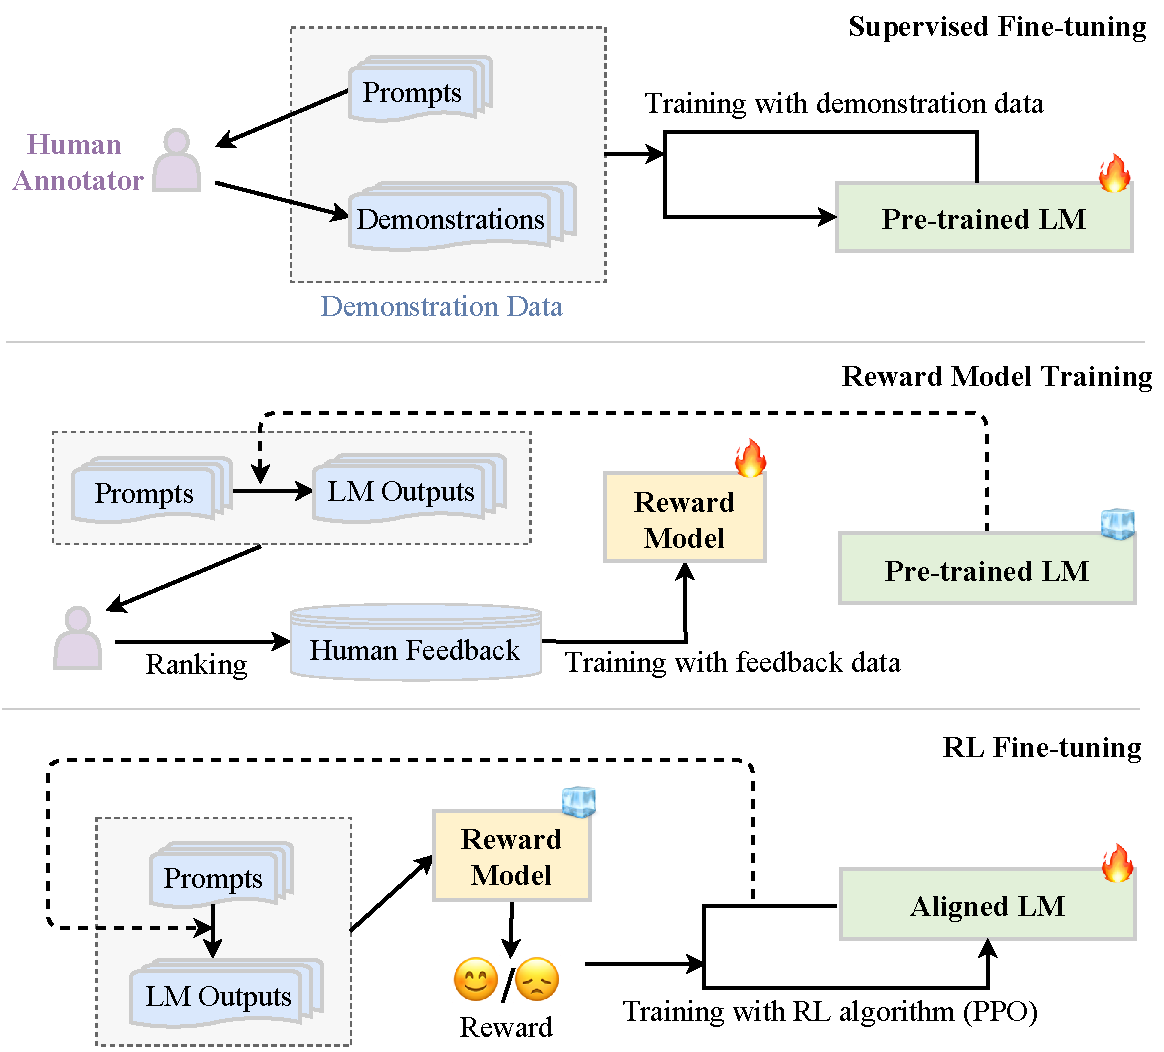
\includegraphics[width=0.5\textwidth]{images/RLHF.pdf}
    \caption{The workflow of the RLHF algorithm.}
    \label{fig:RLHF}
\end{figure}

To align LLMs with human values, reinforcement learning from human feedback (RLHF)~\cite{Christiano-NeurIPS-2017-Deep,Ziegler-arxiv-2019-Fine-Tuning} has been proposed to fine-tune LLMs with the collected human feedback data, which is useful to improve the alignment criteria (\eg helpfulness, honesty, and harmlessness).
RLHF employs reinforcement learning~(RL) algorithms~(\eg Proximal Policy Optimization~(PPO)~\cite{schulman-arxiv-2017-proximal}) to  adapt LLMs to human feedback by learning a reward model. Such an approach incorporates humans in the training loop for developing well-aligned LLMs, as exemplified by InstructGPT~\cite{Ouyang-arxiv-2022-Training}. 

\begin{figure*}[!t]
    \centering
    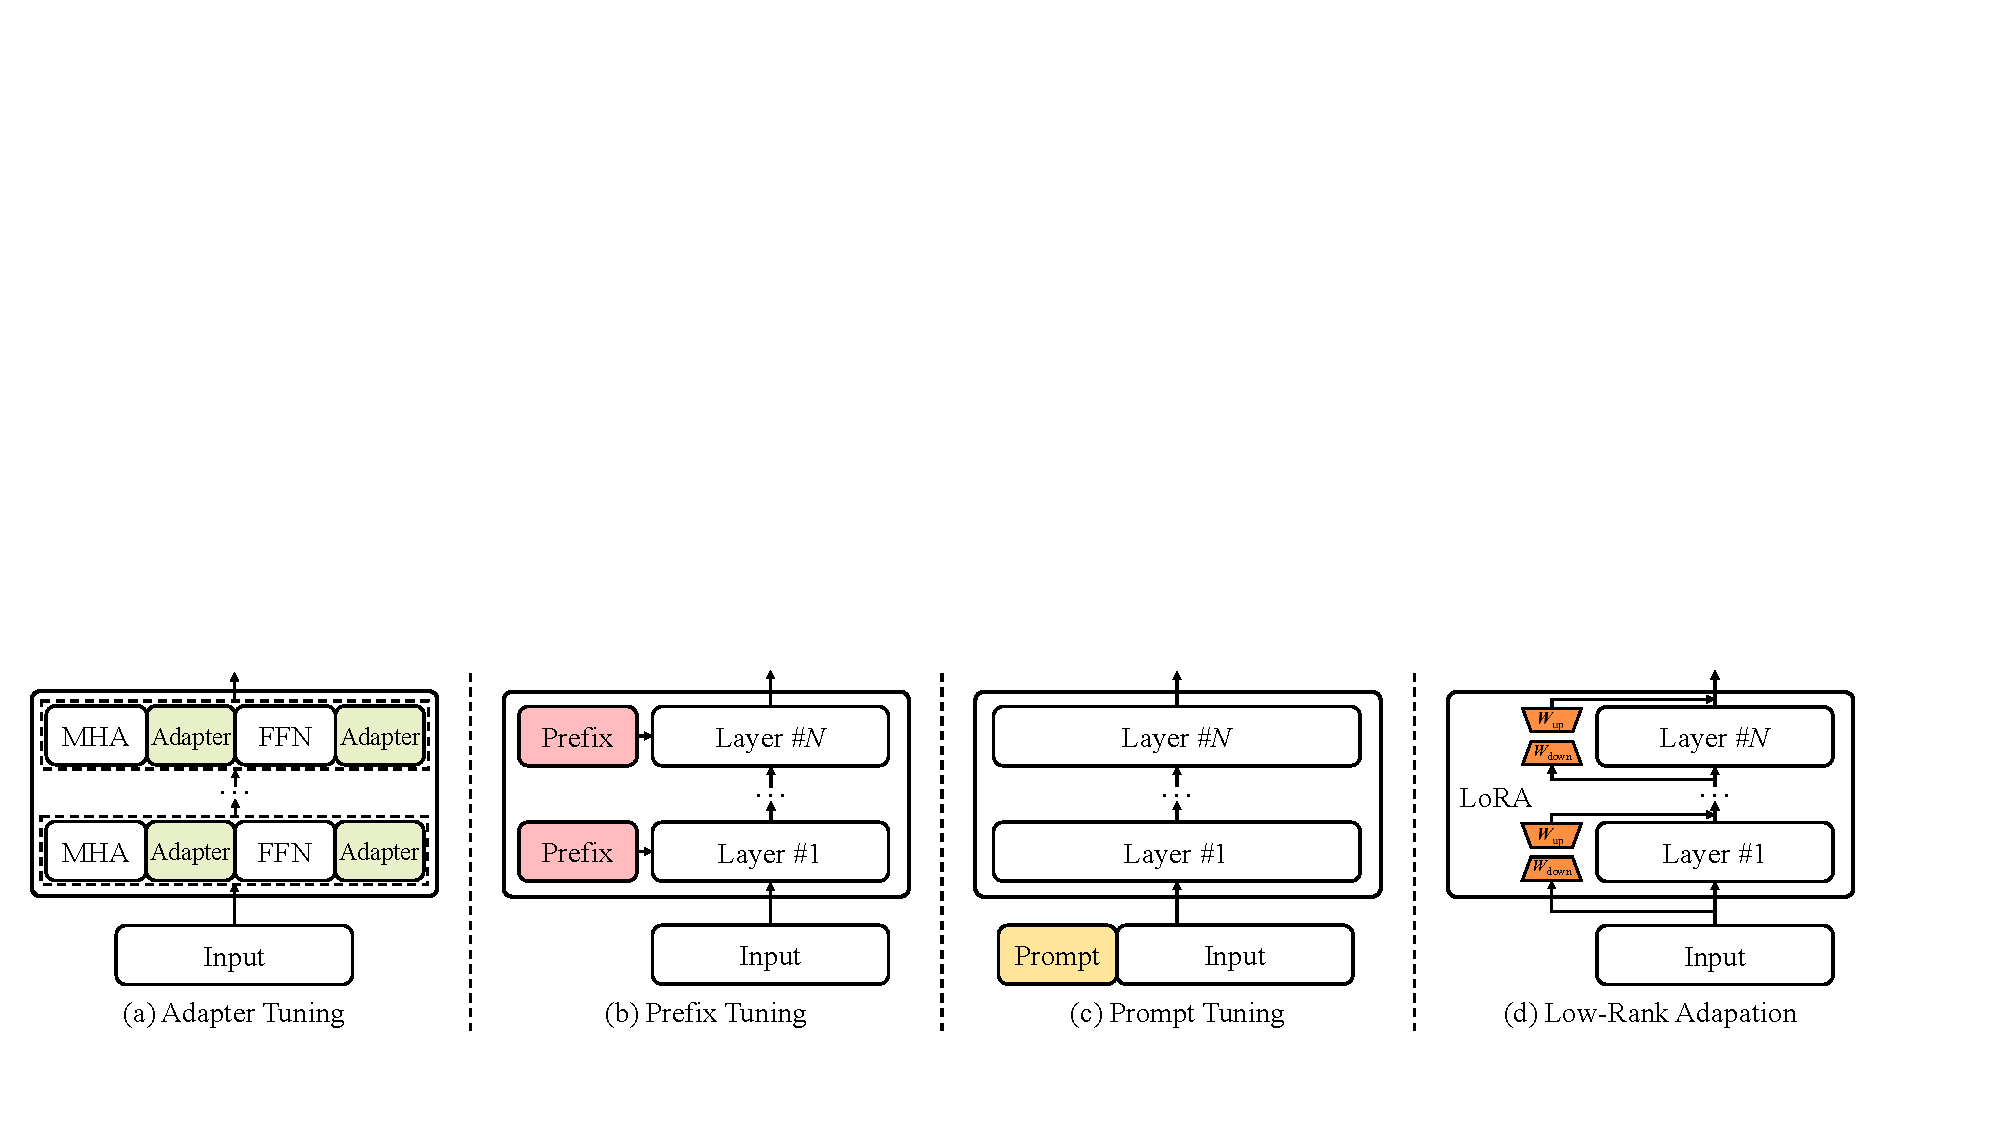
\includegraphics[width=1\textwidth]{images/Efficient-Tuning.pdf}
    \caption{An illustration of four different parameter-efficient fine-tuning methods. MHA and FFN denote the multi-head attention and feed-forward networks in the Transformer layer, respectively.}
    \label{fig:efficient-tuning}
\end{figure*}

\paratitle{RLHF System.}
The RLHF system mainly comprises three key components: a pre-trained LM to be aligned, a reward model learning from human feedback, and a RL algorithm training the LM.  
Specifically, the \textit{pre-trained LM} is typically a generative model that is  initialized with existing pre-trained LM parameters. For example, OpenAI uses 175B GPT-3 for its first popular RLHF model, InstructGPT~\cite{Ouyang-arxiv-2022-Training}, and DeepMind uses the 280 billion parameter model Gopher~\cite{Rae-arxiv-2021-Scaling} for {its GopherCite model~\cite{Menick-arxiv-2022-teaching}. } %
Further, the \textit{reward model~(RM)} provides (learned) guidance signals that reflect human preferences for the text generated by the LM, usually in the form of a scalar value. The reward model can take on two forms: a fine-tuned LM or a LM trained de novo using human preference data.
{Existing work typically employs reward models having  a  parameter scale different from that of the aligned LM~\cite{Menick-arxiv-2022-teaching,Ouyang-arxiv-2022-Training}.} For example, OpenAI uses 6B GPT-3 and DeepMind uses 7B Gopher as the reward model, respectively.
Finally, to optimize the pre-trained LM using the signal from the reward model, a specific \textit{RL algorithm} is designed for large-scale model tuning. Specifically, Proximal Policy Optimization (PPO)~\cite{schulman-arxiv-2017-proximal} is a widely used RL algorithm for alignment in existing work~\cite{Ouyang-arxiv-2022-Training,Menick-arxiv-2022-teaching,Glaese-arxiv-2022-Improving}. 

\paratitle{Key Steps for RLHF.} Figure~\ref{fig:RLHF} illustrates the overall three-step process of RLHF~\cite{Ouyang-arxiv-2022-Training} as introduced below. 

$\bullet$ \textit{Supervised fine-tuning.} To make the LM initially perform desired behaviors, it  usually needs to collect a supervised dataset containing input prompts (instruction) and desired outputs for fine-tuning the LM. These prompts and outputs can be written by human labelers for some specific  tasks while ensuring the diversity of tasks.  
{For example, InstructGPT~\cite{Ouyang-arxiv-2022-Training} asks human labelers to compose prompts (\eg ``\emph{List five ideas for how to regain enthusiasm for my career}'') and desired outputs for several generative tasks such as open QA, brainstorming, chatting, and rewriting. }
Note that the first step is optional in specific settings or scenarios. 

$\bullet$ \textit{Reward model training.} The second step is to train the RM using human feedback data. Specifically, we employ the LM to generate a certain number of output texts using sampled prompts (from either the supervised dataset or the human-generated prompt) as input. We then invite human labelers to annotate the preference for these pairs. The annotation process can be conducted in multiple forms, and a common approach is to annotate by ranking the generated candidate texts, which can reduce  the inconsistency among annotators. Then,  the RM is trained to predict the human-preferred output. In InstructGPT, labelers rank model-generated outputs from best to worst, and the RM (\ie 6B GPT-3) is trained to predict the ranking. Note that, in recent work~\cite{Bai-arXiv-2022-Constitutional}, the annotation of preference on response pairs has been conducted by an AI agent (usually an aligned LLM) instead of humans, which is called ``\emph{reinforcement learning from AI feedback (RLAIF)}''. 
{LLMs trained with typical RLHF algorithms tend to generate harmless responses with less helpfulness, which is  called  \emph{evasion problem}~\cite{Bai-arXiv-2022-Constitutional}. To  guarantee both the harmlessness and helpfulness, RLAIF generates the AI feedback based on pre-set alignment principles in instructions~\cite{Bai-arXiv-2022-Constitutional,Lee-CoRR-2023-RLAIF}, which can also reduce  the efforts of human annotation.} 


$\bullet$ \textit{RL fine-tuning.} At this step, aligning (\ie fine-tuning) the LM is formalized as an RL problem. In this setting, the pre-trained LM acts as the policy that takes as input a prompt and returns an output text, the action space of it is the vocabulary, the state is the currently generated token sequence, and the reward is provided by the RM. To avoid eviating significantly from the initial (before tuning) LM, a penalty term is commonly incorporated into the reward function. 
For example, InstructGPT optimizes the LM against the RM using the PPO algorithm. 
For each input prompt, InstructGPT calculates the KL divergence between the generated results from the current LM and the initial LM as the penalty.
It is noted that the second and final steps can be iterated in multiple turns for better aligning LLMs. 
Due to the instability of the RL algorithm, recent work~\cite{Dong-RAFT-2023-arxiv} replaces the RL tuning with another supervised fine-tuning by reusing the best ranked samples with higher rewards.

\paratitle{Practical Strategies for RLHF.}
{Although RLHF is promising to effectively improve the alignment of LLMs with humans, it is practically challenging for researchers to successfully implement  it.
In this part, we focus on discussing several useful  strategies and tricks for improving the effectiveness and efficiency of RLHF. 
Concretely, we focus on the effective training of reward models, efficient and effective RL training, respectively.}

{$\bullet$ \textit{Effective reward model training.} 
Despite that InstructGPT used a small reward model (6B GPT model), increasing work~\cite{Touvron-2023-llama2-arxiv} has shown it is often more effective to use a large reward model (\eg  equal or greater than the original model size), since large reward models generally perform better in judging the quality of the LLM generated outputs. 
In LLaMa 2~\cite{Touvron-2023-llama2-arxiv},  pretrained chat model checkpoints are used 
to initialize the reward model, they argue that such an approach can effectively reduce the information mismatch between the model to be aligned and the reward model by sharing the same pre-training knowledge.   
Whereas, it is common to encounter the overfitting problem when training large-scale reward models. As a simple yet effective solution, existing work~\cite{askell2021general,zheng2023secrets} has introduced the LM loss on the preferred response of the input prompt from the human-annotated alignment dataset as a regularizer, which alleviates the overfitting of the reward model on the binary classification task. 
In addition, as there are multiple criteria for alignment (\eg helpfulness and honesty), it is often difficult to train a single reward model that can satisfy all the alignment  criteria.
Therefore, it is useful to train multiple reward models that focus on different alignment criteria~\cite{Touvron-2023-llama2-arxiv}, and compute the final reward based on the produced ones from them via special combination strategies (\eg mean pooling and weighted sum).
Such a way enables more  flexible rules or standards on multiple  criteria, \eg  
relaxing the requirement on helpfulness while posing more strict limits on harmfulness.} 

{$\bullet$ \textit{Effective RL training.}
As the RL training process tends to  be unstable and hyper-parameter sensitive,
it is suggested that the language model should be well supervised fine-tuned
 before RL training, so as to reaching a good model capacity.  
A commonly-used way is to fine-tune the LLM on its best outputs of the prompts (referred to as \emph{rejection sampling} or \emph{best-of-$N$}) from the alignment dataset until convergence before RL.
Given a prompt, the LLM would first produce $N$ outputs via the sampling algorithm, and then the best candidate from the model will be selected by the reward model for learning.
After fine-tuning the LLM on the best samples until convergence, the RL  process will be performed to further improve the performance.
LLaMA 2~\cite{Touvron-2023-llama2-arxiv} has successively trained five versions of RLHF models, where the LLM has been progressively improved with the improvement of the reward models.
In this way, the collected prompts and annotations of human preference data can better reflect the issues of the current model checkpoint, thus making special tuning to address these issues. 
In addition, LLaMA 2 also adds samples from prior iterations into the subsequent ones, to alleviate the possible capacity regression issue during iterative optimization.}
 

{$\bullet$ \textit{Efficient RL training.}
As the RL training requires to iterate the inference process of both the LLM and reward models, it would greatly increase the total memory and computation cost, especially for larger reward models and LLMs.
As a practical trick, we can deploy the reward model on a separate server, and invoke the corresponding API to work with the LLM on its own server. 
In addition, as RLHF requires the LLM to generate multiple candidate  outputs, instead of calling the sample decoding procedure for multiple times, it is more efficient to utilize the  beam search decoding algorithm\footnote{\url{https://huggingface.co/docs/transformers/v4.31.0/en/main\_classes/text\_generation\#transformers.GenerationMixin.group\_beam\_search}}.
It only needs to perform one-pass decoding  for response generation, meanwhile such a strategy can also enhance the diversity of the generated candidate responses.  }


\paratitle{Process-Supervised RLHF.} 
{
In existing literature of RLHF~\cite{Uesato-arxiv-2022-Solving}, the supervision signals for RL training can be generally classified into two distinct categories: outcome-supervision signals and process-supervision signals.
The outcome-supervised RLHF employs a quantitative score to assess the quality of the whole text generated by LLMs. In contrast, process-supervised RLHF offers an evaluation of each individual component (\eg sentence, word, or reasoning step) within the generated content, which can provide fine-grained supervision signals to guide the training, helping LLMs refine the  undesired generation contents~\cite{Uesato-arxiv-2022-Solving, Lightman-arxiv-2023-let}.
OpenAI has proposed a fine-grained annotation dataset named PRM800k~\cite{Lightman-arxiv-2023-let} consisting of 12K process-annotated mathematical problems~(\ie MATH dataset~\cite{Hendrycks-nips-2021-Measuring}) and 75K solutions generated by LLMs of these problems, where each reasoning step of mathematical problems is labeled as \emph{positive}, \emph{negative} or \emph{neutral} in PRM800k.
This fine-grained dataset has been utilized in existing work~\cite{Ma-arxiv-2023-Let, Lightman-arxiv-2023-let} to train the process-supervised reward models~(PRM), 
and the probability from the prediction of each label can be considered as the supervision signals during RLHF procedure. 
To effectively leverage process-supervision signals from PRMs, existing work~\cite{Uesato-arxiv-2022-Solving} has utilized expert iteration~\cite{Silver-nat-2017-Mastering,Anthony-nips-2017-Thinking}, an effective RL algorithm to improve the base policy via learning from expert policy.
Typically, expert iteration contains two main stages: policy improvement and distillation~\cite{Uesato-arxiv-2022-Solving}.
In the policy improvement stage, expert policy processes the systematic search procedure to produce the samples.
PRMs provide process-supervision signals to guide expert policy in the search procedure and enhance the quality of samples.
Subsequently, during the distillation stage, the samples generated by expert policy in the first stage are utilized to improve the base policy through supervised fine-tuning.
In addition to expert iteration, PRMs can also be utilized to re-rank the candidates of the final answers generated by LLMs~\cite{Lightman-arxiv-2023-let} or to select  better intermediate reasoning steps during step by step reasoning~\cite{Ma-arxiv-2023-Let, Luo-arxiv-2023-WizardMath}.
}



\subsubsection{Alignment without RLHF}
\label{sec-alignment-withoutRL}

Although RLHF has achieved great success in aligning the behaviors of LLMs with human values and preferences, it also suffers from notable limitations. First, RLHF needs to train multiple LMs including the model being aligned, the reward model, and the reference model at the same time,  which is  tedious in algorithmic procedure and memory-consuming in practice. Besides, the commonly-used PPO algorithm in RLHF is rather complex and often sensitive to hyper-parameters. As an alternative, increasing studies explore to directly optimize LLMs to adhere to human preferences, using supervised fine-tuning without reinforcement learning~\cite{zhou-arxiv-2023-lima}.

\paratitle{Overview.} 
The basic idea of non-RL alignment approaches is to directly fine-tune LLMs with \emph{supervised learning} on high-quality \emph{alignment dataset}.
It basically assumes that response feedback or golden rules to avert unsafe behaviors have been injected or included in the specially curated alignment dataset, so that LLMs can directly learn aligned behaviors from these demonstration data via suitable fine-tuning strategies. 
Thus, to implement this approach, two key issues are the construction of alignment dataset and the design of fine-tuning loss.  %
{For the first issue, the alignment dataset can be automatically constructed by an aligned LLMs according to human-written safety principles~\cite{Sun-arxiv-2023-Principle} or refining existing examples using edits operations~\cite{Liu-NeurIPS-2022-Second}. In addition, we can also reuse existing reward models to select high-rated responses from existing human feedback data~\cite{Dong-RAFT-2023-arxiv}. For the second issue,  non-RL alignment approaches mainly fine-tune  LLMs  in a  supervised learning way (the same as the original instruction tuning loss) on a high-quality alignment dataset, meanwhile auxiliary learning objectives can be used to enhance the  alignment performance, \eg  ranking responses or contrasting instruction-response pairs. } 




\paratitle{Alignment Data Collection.} {The construction of alignment data is important to effectively align the behaviors of LLMs with human preferences. To collect high-quality alignment data, 
some work tries to reuse existing reward models to {select} high-rated  responses,  and others explore to leverage powerful LLMs (\eg ChatGPT) or build a simulated environment to generate synthetic alignment examples. Next, we will discuss these three lines of research.
}

$\bullet$  {\textit{Reward model based approaches.} The reward model in RLHF has been trained to measure the alignment degree on {the responses of LLMs}. It is straightforward to leverage existing reward models to select high-quality responses as alignment data for subsequent fine-tuning. Based on this idea, RAFT~\cite{Dong-RAFT-2023-arxiv} adopts reward models trained on human preference data to rank the responses of LLMs and collect those with higher rewards for supervised fine-tuning. 
In addition, the reward model can be also used to score model responses and assign them to different quality groups. Quark~\cite{Lu-nips-2022-quark} sorts the responses of LLMs into different quantiles based on the reward scores. Each quantile is attached with a special reward token to represent the reward level of the quantile. Conditioned on the highest-reward tokens, LLMs are subsequently prompted to generate high-quality responses. {Given an initial answer and the corresponding human feedback, ILF~\cite{Scheurer-arxiv-2023-ILF} first adopts LLMs to generate refined answers, then utilizes the reward model to select the answer that best matches the feedback for further training.}
As valuable resources for aligning LLMs, several reward models have been released, including DeBERTa-base/large/xxlarge from OpenAssistant\footnote{https://huggingface.co/OpenAssistant}, Moss-7B from Fudan\footnote{https://github.com/OpenLMLab/MOSS-RLHF}, and Flan-T5-xl from Stanford\footnote{https://huggingface.co/stanfordnlp/SteamSHP-flan-t5-xl}.



$\bullet$ {\textit{LLM based generative approaches.} Reward models help to select aligned data from model responses. However, training reward models itself necessitates substantial high-quality human-labeled data, which is typically expensive and in short supply. 
In addition, although existing reward models can be reused, they might not be able to accurately capture the nonalignment behaviors in another separately trained LLM.   
Therefore, some work explores leveraging powerful LLMs to automatically generate human-aligned data. As a representative work, constitutional AI~\cite{Bai-arXiv-2022-Constitutional} proposes  that human supervision comes from a set of principles (\ie natural language instructions) governing AI behaviors. Based on these principles, LLMs will critique their own harmful responses and revise them repeatedly into finally aligned responses. Similarly, Self-Align~\cite{Sun-arxiv-2023-Principle} first adopts self-instruct~\cite{Wang-arXiv-2022-Self} to generate instructions focusing on covering diverse topics. Then, the model is also prompted with multiple human-written principles that describe the rules of expected model behaviors (also with several in-context exemplars), to generate helpful, ethical, and reliable responses as alignment data. 
{To mitigate the limit that the original SFT method can only learn from positive responses, 
FIGA~\cite{Guo-arxiv-2023-Beyond} develops an improved supervised alignment approach, where both  negative (the original output of low quality) and positive (the refined output by LLMs) responses are leveraged in a contrastive way, to enable LLMs to deeply understand what fine-grained revisions actually  lead to good response. 
}


$\bullet$ {\textit{LLM based interactive approaches.} Most existing approaches train LLMs in isolation, where LLMs are not present in actual  environments to improve themselves through external feedback signals. As a comparison, humans learn social norms and values from interactions with others in social environments~\cite{Krishna-PNAS-2022-Socially}. To mimic such a learning approach, Stable Alignment~\cite{Liu-arxiv-2023-training} builds a simulated interaction environment  consisting of a number of LLM agents, where AI agents keep interacting with and  each other, receiving feedback on improvement.  
Once a central agent receives an instruction, it produces a response and shares it with nearby agents. These critic  agents generate feedback comprising ratings about the response and revision  suggestions. Then the central agent would revise the original response following these suggestions. %
}
Such an alignment approach can be also extended to real-world environment with humans. 
 
\paratitle{Supervised Alignment Tuning.} {After obtaining alignment data,} it is also key to design suitable fine-tuning strategies for direct alignment. A straightforward approach is to optimize LLMs  using the conventional sequence-to-sequence objective based on the alignment data. 
In addition to the conventional optimization objective, several studies further explore auxiliary losses that enhance the learning from the alignment data.}

$\bullet$ \textit{Primary training objective.} Since the alignment data typically consists of an input instruction and an output response, the primary training loss is still the traditional cross-entropy loss for sequence-to-sequence learning. Based on this loss, many studies propose a number of improvement variants for enhancing the supervised alignment tuning. For example, CoH~\cite{Liu-arxiv-2023-Chain} constructs the training data by prepending ``\emph{A helpful answer:}'' and ``\emph{An unhelpful answer:}'' to the annotated good and bad responses, respectively, and only compute losses for those response tokens with special masking.  Quark~\cite{Lu-nips-2022-quark} sorts model responses into different quantiles with varying alignment quality, it prepends a special reward token to each model response to represent the reward level of the response. Further, to enable the preference modeling via the maximum likelihood objective, DPO~\cite{Rafailov-arxiv-2023-Direct} first reparameterizes the response rewards using the policy model (\ie the language model being optimized), and then the original reward modelling objective can be reformulated only based on the policy model. In this way, DPO removes the explicit reward modeling step, and optimizing the new learning objective only involving the policy model is equivalent to optimizing the rewards. 
{Furthermore, FIGA~\cite{Guo-arxiv-2023-Beyond} designs a fine-grained contrastive loss that aims to encourage desirable tokens, penalize undesirable ones, and disregard trivial tokens.}


$\bullet$ \textit{Auxiliary optimization objectives.} Besides the primary cross-entropy loss, several studies propose auxiliary training loss to enhance the learning from the alignment data. First, since the responses of each instruction can be scored by the reward model, the ranking loss can be used to train the model to preserve the ranking order of these responses. For example, RRHF~\cite{Yuan-RRHF-2023-arxiv} samples responses from multiple sources, including model-generated responses, such as those derived from the model itself, ChatGPT, and GPT-4, as well as human-written responses, spanning both high-quality and low-quality instances.   To align with the scores from reward models, it further optimizes the ranking loss by encouraging the model to have a higher conditional log probability for the response with a higher ranking.  {SLiC-HF~\cite{Zhao-arxiv-2023-slichf} proposes to assess the similarity between model outputs and human preference via the distance in the latent space,  and introduces specific calibration and regularization loss to calibrate the candidate sequences based on human-preference data.} Second, to enhance the relatedness between the response and the instruction, some work adopts contrastive learning to push up the probability of correct instruction-response pairs while pushing down incorrect instruction-response pairs. Specifically, for an output response, the proposed approach in \cite{Zhang-arxiv-2023-The} contrasts the target instruction to the other irrelevant instructions. By doing so, it can enable the model to learn the right correlation between instructions and responses.





%


\subsubsection{Remarks on SFT and RLHF}
\label{sec-remarks-SFTRL}
As discussed in Section~\ref{sec-instruction}, instruction  tuning is the process of training pre-trained language models with
formatted demonstration data (instructions paired with desired outputs). At early exploration,   instruction data was mainly collected from NLP  tasks~\cite{Wei-ICLR-2022-Finetuned}, while it has been now extended to more diverse supervision data  that pairs input and output texts (\eg the utterances of open-ended dialogues). Training with such paired texts is also  called \emph{supervised fine-tuning~(SFT)} in the context of LLMs~\cite{Ouyang-arxiv-2022-Training}. 
In this part, we mainly use the abbreviation  \emph{SFT} for discussion but not instruction tuning, due to the simplicity and popularity. 

Since SFT and RLHF are two major adaptation tuning methods for LLMs, it is important to understand the connections and difference between them.  
Next, we make some discussions on this issue\footnote{This part would be somehow subjective, mainly based on the authors' opinions and experiences. Comments or corrections are welcome to enhance this part. }.

\paratitle{Overall Comparison with RL Formulation}. Following the discussion in Section~\ref{sub:RLHF} (the part related to RL training),  the text generation problem can be formulated as a decision-making process based on RL. 
Taking a prompt as input, the task of a LLM is to generate a text completion that appropriately responds to the prompt. This task would be completed step by step. At each step, an  agent (\ie LLM) will perform an action (\ie generating a token) according to the policy (\ie the generative probability distribution of LLM) conditioned on the current state (currently generated token sequence and other available  context information). 
It is expected that a high-quality output text would be produced by the LLM, which can earn a large reward score based on the entire response.  
Overall, RLHF and SFT can be considered as two different training approaches to optimizing  the  above decision making process for LLMs.     
Specially, RLHF 
firstly learns the reward model, and then employs it to improve the LLM with RL training (\eg PPO). As a comparison, SFT adopts  a teacher-forcing approach, which directly optimizes the likelihood of  a demonstration output. 
Such a token-level training way essentially does  \emph{behavior cloning} (a special algorithm of imitation learning~\cite{Ahmed-ACM-2017-Imitation}): it utilizes the expert's action (\ie the target token at each step) as the supervision label and directly learns to imitate the demonstrations from experts without specifying a reward model as in typical RL algorithms. 
To learn the desired policies, 
SFT adopts a ``local'' optimization way (\ie token-level loss) based on demonstration data, while RLHF takes a  ``global'' optimization way (\ie text-level loss) by involving human preference. More theoretical analysis about  imitation learning and reinforcement learning can be referred to the related RL literature \cite{Ahmed-ACM-2017-Imitation,Levine-youtube-2022-Imitate}.  


%

\paratitle{Pros and Cons of SFT}.  
SFT has been shown to be an effective approach to  boosting the performance of LLMs on various  benchmarks~\cite{Wei-ICLR-2022-Finetuned,Chung-arxiv-2022-Scaling,alpaca,vicuna2023}, which can largely enhance the task generalization ability  and  flexibly endow specific functions (\eg establishing the chatbot's identity). 
More discussions about the usefulness of SFT can be found in Section~\ref{subsec:effectIT}.  
It has been  widely recognized  that SFT mainly \emph{unlocks} the abilities but not \emph{inject} new abilities into LLMs.   
Thus, it might become problematic when one tries to stimulate the non-endogenous abilities of LLMs via SFT.  %
As a concrete scenario, it would potentially advocate the  hallucination behaviors when demonstration data is beyond the knowledge or ability scope of LLMs, \eg training a LLM to answer questions about its unknown facts.   
An interesting viewpoint from John Schulman's talk on RLHF~\cite{John-youtube-2023-RLHF} is that distilling superior models to train less capable models (\eg prompting GPT-4 to generate the response as fine-tuning data) might increase the possibilities of generating the hallucinated texts, thus likely affecting the factual accuracy of LLMs. 
Furthermore, as a behavior cloning method, SFT aims to imitate the behaviors (without explorations) of the experts who construct the demonstration data. 
However, there often exist variations among different annotators on the writing styles, quality, and preferences of demonstration data, which tends to affect the learning performance of SFT. 
Thus, high-quality instruction data (but not the quantity) is the primary factor for effective training of LLMs during the SFT stage~\cite{Touvron-2023-llama2-arxiv}.  %

\paratitle{Pros and Cons of RLHF}. %
RLHF was early explored in the literature of deep RL~\cite{Christiano-NeurIPS-2017-Deep},  then  borrowed to improve the capacity of language models (\eg summarization~\cite{Stiennon-arxiv-2020-learning}), and subsequently adopted as the fundamental  technique  to develop InstructGPT~\cite{Ouyang-arxiv-2022-Training}. Recently, increasing evidence~\cite{Touvron-2023-llama2-arxiv,Bai-arXiv-2022-Constitutional} has  demonstrated the effectiveness of RLHF in mitigating the  harmful responses and enhancing the model capacity. 
Specially, LLaMA 2 has demonstrated that RLHF can improve both the helpfulness and harmlessness scores~\cite{Touvron-2023-llama2-arxiv}, and  attributed this to a better human-LLM synergy for data annotation. 
They explain this reason in two major aspects as follows. 
First, since human annotators mainly provide preference annotations for RLHF, 
it can largely alleviate the discrepancies of annotators as that in SFT. Secondly, 
preference annotation is much easier than writing the demonstration data, and annotators can even judge the quality of more superior generations than those they create, making it possible to explore a broader state space beyond what can be demonstrated by human annotators. 
Another key point is that RLHF essentially encourages LLMs to learn correct policies by contrasting the  self-generated responses (discriminating between good and bad responses). It no longer forces the model to imitate external demonstration data, and thus can mitigate the hallucination issues with SFT as discussed above\footnote{In RLHF,  it seems to be also important  that reward models should be aware of the knowledge or ability of a LLM to be aligned. For example, LLaMA 2 adopts pre-trained chat model checkpoints  to initialize reward models~\cite{Touvron-2023-llama2-arxiv}. }. Actually, RLHF has been demonstrated to be an important approach to reduce the  hallucination behaviors in GPT-4~\cite{OpenAI-OpenAI-2023-GPT-4}.  
However, RLHF inherits the drawbacks of classic RL algorithms, \eg sample  inefficiency and training instability. 
When adapted to LLMs, RLHF further  relies on a strong SFT model as initial model checkpoint for efficiently achieving good performance.
In addition, human annotators are involved in a complex iterative optimization process, in which a number of important details (\eg the prompt selection, the schedule of reward model training and PPO training, and the settings of hyper-parameters) have important impact on the whole model performance.   

Overall, SFT is particularly useful to increase the model capacity of pre-trained model checkpoints right after pre-training, while RLHF is promising to further improve the model capacity of SFT models. However, RLHF has been difficult to implement, and far from well explored (according to public literature), and more improvements (\eg efficient and reliable annotation~\cite{Bai-arXiv-2022-Constitutional} and simplified optimization~\cite{Rafailov-arxiv-2023-Direct}) are still needed for further   research. 









\subsection{Parameter-Efficient Model Adaptation}\label{sec-PEFT}
In the above, we have discussed the approaches of instruction tuning and alignment tuning to adapt LLMs according to specific goals. Since  LLMs consist of a huge amount of model parameters, it would be costly to perform the full-parameter tuning. In this section, we will discuss how to conduct efficient tuning  on LLMs.  We first review several representative parameter-efficient fine-tuning methods for Transformer language models, and then summarize existing work on parameter-efficient fine-tuned LLMs. 

\subsubsection{Parameter-Efficient Fine-Tuning Methods}\label{sec-PEFT-methods}
In existing literature, parameter-efficient fine-tuning~\cite{Li-ACL-2021-prefix,Lester-ACL-2021-The,Hu-ICLR-2022-LoRA} has been an important topic that aims to reduce the number of trainable parameters while retaining a good performance as possible. In what follows, we briefly review four  parameter-efficient fine-tuning methods for Transformer language models, including adapter tuning, prefix tuning, prompt tuning and 
LoRA. The illustration of these four methods are shown in Figure~\ref{fig:efficient-tuning}.


\paratitle{Adapter  Tuning}. Adapter tuning  incorporates small neural network modules (called \emph{adapter}) into the Transformer models~\cite{Houlsby-ICML-2019-Parameter}. To implement  the adapter module, a bottleneck architecture has been proposed in \cite{Houlsby-ICML-2019-Parameter,Hu-arXiv-2023}, which first compresses the original feature vector into a smaller dimension (followed by a nonlinear transformation) and then recovers it to the original dimension.  
The adapter modules would be integrated into each Transformer layer, typically using a serial insertion after each of the two core parts (\ie  attention layer and feed-forward layer) of a Transformer layer. 
Alternatively,  parallel adapters~\cite{He-ICLR-2022-towards} can be also used in Transformer layers, where it places two adapter modules in parallel with the attention layer and feed-forward layer accordingly.   
During fine-tuning, the adapter modules would be optimized according to the  specific task goals, while the parameters of the original language model are  frozen in this process. 
In this way, we can effectively reduce the number of trainable parameters during fine-tuning.


\paratitle{Prefix Tuning}. 
Prefix tuning~\cite{Li-ACL-2021-prefix} prepends a sequence of prefixes, which are a set of trainable continuous vectors,  to each Transformer layer in language models.  These prefix vectors are task-specific,  which can be considered as virtual token embeddings. To optimize the prefix vectors, a reparameterization trick~\cite{Li-ACL-2021-prefix} has been proposed by learning a MLP function that maps a smaller matrix to the parameter matrix of prefixes, instead of directly optimizing the prefixes.   
It has been shown that this trick is useful for stable training.  
After optimization, the mapping function would be discarded, and only the derived prefix vectors are kept to enhance task-specific performance. 
Since only the prefix parameters would be trained, it can lead to a  parameter-efficient model optimization.
Similar to prefix tuning, p-tuning v2~\cite{Liu-arXiv-2021-P-tuning} incorporates layer-wise prompt vectors into the Transformer architecture specially for natural language understanding, which also utilizes multi-task learning for jointly optimizing shared prompts.  
It has been shown to be useful in improving the model performance of different  parameter scales  on  natural language understanding tasks. 




\paratitle{Prompt Tuning}. Different from prefix tuning, prompt tuning~\cite{Liu-arXiv-2021-GPT,Lester-ACL-2021-The}  mainly focuses on incorporating trainable prompt vectors at the input layer\footnote{Here, prompt tuning denotes a category of related efficient tuning methods exemplified by the work~\cite{Liu-arXiv-2021-GPT,Lester-ACL-2021-The,gu-ACL-2022-ppt}, instead of a specific method as used in \cite{Lester-ACL-2021-The}. Indeed, the prefix based tuning methods~\cite{Li-ACL-2021-prefix,Liu-arXiv-2021-P-tuning} can be also considered as prompting methods, which are called \emph{deep prompting tuning}   in \cite{Liu-arXiv-2021-P-tuning}. In this survey, prompt tuning specially refer to the methods that only include the prompt tokens at the input layer, in the context of LLMs.
We assign p-tuning v2~\cite{Liu-arXiv-2021-P-tuning} to the category of prefix tuning, because it incorporates layerwise prompts in langauge models. }. 
Based on the discrete prompting methods~\cite{jiang-TACL-2020-how,shin-EMNLP-2020-autoprompt}, it  augments the input text  by including a group of soft prompt tokens (either in a free form~\cite{Liu-arXiv-2021-GPT} or a prefix form~\cite{Lester-ACL-2021-The}), and then takes the prompt-augmented input to solve specific downstream tasks. 
In implementation, task-specific prompt embeddings are combined with the input text embeddings, which are subsequently fed into language models. P-tuning~\cite{Liu-arXiv-2021-GPT} has proposed a free form to combine the context, prompt and target tokens, which can be applied to the  architectures for both natural language understanding and generation. They further learn the representations of soft prompt tokens by a bidirectional LSTM. 
Another representative approach~\cite{Lester-ACL-2021-The}  named \emph{prompt tuning} directly prepends  prefix prompts to the input.
During training, only the prompt embeddings would be learned according to  task-specific supervisions.
Since this method only includes a small number of trainable parameters at the input layer, it has been found that the performance highly relies on the model capacity of the underlying language models~\cite{Lester-ACL-2021-The}.  




\paratitle{Low-Rank Adaptation~(LoRA)}. LoRA~\cite{Hu-ICLR-2022-LoRA} imposes  the low-rank constraint for approximating the update matrix at each dense layer, so as to reduce the trainable parameters  for adapting to downstream tasks. 
Consider the case of optimizing a parameter matrix $\mathbf{W}$. The update process can be written in a general form as:   $\mathbf{W} \leftarrow \mathbf{W} + \Delta \mathbf{W}$. 
The basic idea of LoRA is to freeze the original matrix $\mathbf{W} \in \mathbb{R}^{m \times n}$ while approximating the parameter update $\Delta \mathbf{W}$ by low-rank decomposition matrices, \ie $\Delta \mathbf{W}=\mathbf{A}\cdot  \mathbf{B}^\top$, where $\mathbf{A}\in \mathbb{R}^{m \times k}$ and $\mathbf{B}\in \mathbb{R}^{n \times k}$ are the trainable  parameters for task adaptation and $k \ll \min(m,n)$ is the reduced rank. The major merit of LoRA is that it can largely save the memory and storage usage (\eg VRAM). Further, one can only keep a single large model copy, while maintaining a number of task-specific low-rank decomposition matrices for adapting to different downstream tasks.
Further, several studies have also discussed how to set the rank in a more principled approach, \eg  importance score based allocation~\cite{Zhang-arXiv-2023-Adaptive} and search-free optimal rank selection~\cite{Valipour-arXiv-2022-DyLoRA}.

Besides the above  methods, there is  extensive research on efficient tuning of Transformer language models.  
 However, a more comprehensive discussion  of efficient tuning is beyond the scope of this article, which can be found in the related papers on this topic~\cite{He-ICLR-2022-towards,Ding-NMI-2023-Parameter}.  
 



\subsubsection{Parameter-Efficient Fine-Tuning on LLMs}
With the rising of LLMs, efficient tuning  has attracted increasing research attention for developing a more lightweight adaptation approach in downstream tasks. 


In particular, LoRA~\cite{Hu-ICLR-2022-LoRA} has been widely applied to open-source LLMs (\eg LLaMA and BLOOM) for parameter-efficient fine-tuning. 
Among these research attempts, LLaMA and its  variants have  gained much attention for parameter-efficient tuning.  
For example, Alpaca-LoRA~\cite{Alpaca-LoRA} has been trained using LoRA as a lightweight tuned  version of  Alpaca~\cite{Taori-github-2023-Stanford} (a fine-tuned 7B LLaMA model with 52K human demonstrations of instruction following).  
There are extensive explorations of Alpaca-LoRA ranging in different languages or model sizes, which can be found in the collection page\footnote{https://github.com/tloen/alpaca-lora}. 
 A recent study LLaMA-Adapter~\cite{Zhang-arXiv-2023-LLaMA-Adapter} inserts  learnable prompt vectors into each Transformer layer, in which zero-initialized attention has been proposed to improve the training by mitigating the influence of under-fitted prompt vectors. They  also extend this approach to a multi-modal setting, \eg visual question answering.   

Further, an empirical study~\cite{Hu-arXiv-2023} has been conducted to examine the effect of  different tuning methods on  language models.
They compare four efficient tuning methods including  serial adapter tuning~\cite{Houlsby-ICML-2019-Parameter},  parallel adapter tuning~\cite{He-ICLR-2022-towards,Pfeiffer-EMNLP-2022-MAD-X}, and LoRA~\cite{Hu-ICLR-2022-LoRA}, on three open-source LLMs,   namely GPT-J (6B), BLOOM (7.1B) and LLaMA (7B), for evaluation.  Based on the experimental results on six math reasoning datasets, they show that these efficient-tuning methods  under-perform the reference baseline GPT-3.5 on difficult tasks, while achieving a comparable performance on simple tasks. 
Overall, LoRA performs relatively  well among these  comparison methods, using significantly fewer trainable parameters.     

As an important resource, the library \emph{PEFT}~\cite{peft-github-2022} (standing for parameter-efficient fine-tuning) has been released on GitHub\footnote{https://github.com/huggingface/peft}. It has included several widely used efficient tuning methods, including LoRA~\cite{Hu-ICLR-2022-LoRA}/AdaLoRA~\cite{Zhang-arXiv-2023-Adaptive}, prefix-tuning~\cite{Li-ACL-2021-prefix,Liu-arXiv-2021-P-tuning}, P-Tuning~\cite{Liu-arXiv-2021-GPT}, and prompt-tuning~\cite{Lester-ACL-2021-The}. Further, it supports a number of language models such as GPT-2 and LLaMA, and also covers several representative vision Transformer models (\eg ViT and Swin Transformer).       


As  discussed in Section~\ref{sec-PEFT-methods}, there have been a large number of efficient tuning methods proposed in the existing literature. However,  most of these approaches are tested on  small-sized pre-trained  language models, instead of the LLMs. 
So far, there still lacks a thorough investigation on the effect of  different efficient tuning methods  on large-sized language models at different settings or tasks.  








\subsection{Memory-Efficient Model Adaptation}\label{sec-memory}  

Due to the huge number of model parameters, LLMs take a significant memory footprint for inference, making it very costly to be deployed in real-world applications. In this section, we discuss how to reduce the memory footprint of LLMs via a popular model compression approach (\ie model quantization), so that large-sized LLMs can be used in resource-limited settings, which also likely reduces the inference latency.  


\subsubsection{Background for Quantization} In this part,  we 
present a general introduction of quantization techniques for neural networks. 

In neural network compression, quantization often refers to the mapping process from  floating-point numbers to  integers~\cite{Gholami-CoRR-2022-A}, especially the 8-bit integer quantization (\ie  \emph{INT8 quantization}). 
For neural network models, there are typically two kinds of data to be quantized, namely \emph{weights} (model parameters) and \emph{activations} (hidden activations), which are originally represented in floating-point numbers.  To illustrate the essential idea of model quantization,  we   introduce a simple yet popular quantization function:
$x_q = R(x/S) - Z$, which transforms a floating number $x$ into a quantized value $x_q$. In this function, 
$S$ and $Z$ denote the scaling factor (involving two  parameters $\alpha$ and $\beta$ that determine the clipping range) and zero-point factor (determining symmetric or asymmetric quantization),  respectively, and $R(\cdot)$ denotes the rounding operation that maps a scaled floating value to an approximate integer. 


As the reverse process,  \emph{dequantization}  recovers the original value from the quantized value accordingly: $\Tilde{x} = S\cdot (x_q + Z)$.  The  quantization error is calculated as the numerical difference between the original value $x$ and the recovered value $\Tilde{x}$.  
{The range parameters  $\alpha$ and $\beta$ have a large impact on the quantization  performance}, which often need to be  \emph{calibrated} according to real data distributions, in either a \emph{static} (offline) or \emph{dynamic} way (runtime).

For more details, we refer to the readers to the excellent  survey~\cite{Gholami-CoRR-2022-A} about quantization methods on neural networks.  




\subsubsection{Quantization Methods for LLMs}

There are generally two major model quantization approaches, namely \emph{quantization-aware training~(QAT)}~(requiring additional full model retraining) and \emph{post-training quantization~(PTQ)} (requires no model retraining). 
Compared with small-sized language models, two major differences need to be considered when designing or selecting quantization methods for LLMs. Firstly, LLMs consist of a huge number of parameters, and thus PTQ methods are more preferred due to a much lower computational cost than QAT methods. Secondly, LLMs exhibit very different activation patterns (\ie large outlier features), and it becomes more  difficult to quantize LLMs, especially  hidden activations. Next, we will briefly review several representative PTQ  methods\footnote{Since we mainly focus on discussing  quantization methods in the context of LLMs,  the line of  quantization work on small-sized language models (\eg BERT) has not been included in this survey. 
} for LLMs.   


\paratitle{Post-Training Quantization~(PTQ)}. We first introduce the PTQ methods for LLMs. 


$\bullet$ \emph{Mixed-precision decomposition}. 
As observed in \cite{Dettmers-arxiv-2022-LLM}, extreme large values occur in hidden activations (called \emph{the emergence of outliers}) when the model size reaches  6.7B parameters or above. %
Interestingly, these outliers are mainly distributed in  some specific  feature dimensions  at Transformer layers. 
Based on this finding, a vector-wise  quantization approach, called \emph{LLM.int8()}, has been proposed in \cite{Dettmers-arxiv-2022-LLM}, which separates  the feature dimensions with outliers and the rest dimensions  in  matrix multiplication. 
Then, the calculations for the two parts are performed with \emph{16-bit floating numbers} and \emph{8-bit integers}, respectively, so as to recover these outliers in a high precision. 

$\bullet$ \emph{Fine-grained quantization}.
For Transformer models, weights and activations are usually represented in the form of tensors. A straightforward approach is to use coarse-grained   quantization parameters for the  whole tensor (\ie  per-tensor quantization)~\cite{Xiao-CoRR-2022-SmoothQuant}. However, it usually leads to inaccurate reconstruction results. 
Thus, fine-grained  methods are proposed to reduce the quantization error.  %
ZeroQuant~\cite{Yao-NeurlPS-2022-ZeroQuant} adopts a  token-wise quantization approach with dynamic calibration for compressing activations. Whereas for weights (easier to be quantized), it uses a group-wise quantization. In practice, a group size of 128~\cite{Yao-NeurlPS-2022-ZeroQuant,Lin-arXiv-2023-AWQ} is commonly used for model quantization.  %









$\bullet$ \emph{Balancing the quantization difficulty}.   
Considering that weights are easier to be quantized than activations, SmoothQuant~\cite{Xiao-CoRR-2022-SmoothQuant}  proposes to migrate the difficulty from  activations to weights. Specially, they incorporate a scaling transformation  to balance the difficulty between weights and activations in a linear layer: $\mathbf{Y} = (\mathbf{X}\text{diag}(\mathbf{s})^{-1}) \cdot (\text{diag}(\mathbf{s})\mathbf{W})$. %
By introducing an mathematically equivalent transformation, this formula  controls the quantization difficulty through the scaling factor $\mathbf{s}$. 
To set $\mathbf{s}$, it  incorporates a migration strength parameter $\alpha$ to balance the difficulties,  where each entry $s_j=\max(\mathbf{x}_j)^\alpha / \max(\mathbf{w}_j)^{(1-\alpha)}$ is determined by  the migration strength.  %



{
$\bullet$ \emph{Layerwise quantization}. This approach finds optimal  quantized weights that minimize a layerwise reconstruction loss: {$\arg\min_{\widehat{\mathbf{W}}}\parallel \mathbf{W}\mathbf{X} -  \widehat{\mathbf{W}} \mathbf{X}\parallel_2^2$}.  %
To efficiently optimize this objective, GPTQ~\cite{frantar-arxiv-2022-gptq} improves the  original optimal brain quantization~(OBQ)~\cite{Frantar-NeurIPS-2022-Optimal} method by fixing the quantization order of weights for all rows. 
Further, with specially designed   methods (\ie lazy batch-updates and Cholesky reformulation),  GPTQ  is feasible to quantize very large models (\eg 175B OPT)  in 3 or 4 bit precision.   
More recently, AWQ~\cite{Lin-arXiv-2023-AWQ} further simplifies the optimization form by incorporating activation-aware scaling for weights, which resembles the idea of  SmoothQuant~\cite{Xiao-CoRR-2022-SmoothQuant}: weights corresponding to outlier activations are more important to be precisely quantized. It does not directly optimize the reconstruction loss, but instead performs simple hyper-parameter search to achieve  the minimal  loss on calibration data. 
}

%


  


%


These strategies in the above methods can be jointly used to improve the quantization performance. 
{In order to achieve high-efficiency implementation, quantization methods also rely on hardware- or system-level support (\eg efficient GPU kernels or hardware-friendly group partition). %
} 


\paratitle{Other Quantization Methods}. In the above, we mainly focus on PTQ methods, and next introduce two recent studies that explore efficient fine-tuning methods or QAT methods   for quanitizing LLMs. 
   

$\bullet$ \emph{Efficient fine-tuning enhanced quantization.} 
For post-training quantization, direct low-bit  quantization (\eg INT4 quantization) often results in large performance degradation.  To overcome this challenge, QLoRA~\cite{Dettmers-CoRR-2023-QLoRA} 
incorporates additional small tunable  adapters (16-bit precision) into the quantized models,  to achieve an efficient, high-precision model fine-tuning.  
It combines the merits of LoRA~(See Section~\ref{sec-PEFT-methods}) and quantization methods. The experiment results show that 4-bit quantized  models can 
achieve the full 16-bit fine-tuning performance by QLoRA.



$\bullet$ \emph{Quantization-aware training~(QAT) for LLMs}. A recent study~\cite{liu-2023-arxiv-LLM-QAT} explores the effect of QAT methods by applying a data-free distillation method to compress the weights, activations as well as key-value cache. By conducting extensive experiments based on LLaMA, they show promising results with 4-bit quantization on both weights and key-value cache, but not on 4-bit activation quantization, which still needs more exploration. 





\subsubsection{Empirical Analysis and Findings}
\label{sec:quantization_empirical}
Quantization has currently become a common technique to reduce the memory footprint and latency of LLMs in deployment. 
In particular, it is important to understand what level of precision (\eg INT8 or INT4) can be applied to quantize different parts of LLMs (\eg weights or activations), while retaining  a high accuracy. 
In this part, we first summarize the major findings about the quantization of LLMs in existing literature, and then present some empirical analysis with quantization experiments.  

\paratitle{Important Findings from Existing Work}. Recently, a very comprehensive evaluation~\cite{Yao-CoRR-2023-ZeroQuant-V2}  has been conducted about the impact of multiple factors (\eg model size and sensitivity) on the post-training quantization methods. Another  study~\cite{Dettmers-2022-arxiv-case} examines the scaling law of $k$-bit quantization in inference performance.   
{In addition to  the overall performance, the study~\cite{Liu-2023-arxiv-Do_emergent} specifically focuses on the potential impact of quantification on emergent capabilities, as well as the levels of performance that can be achieved across various levels of bit precision.}
Also,  prior  work (\eg LLM.int8()~\cite{Dettmers-CoRR-2022-LLM.int8}, GPTQ~\cite{frantar-arxiv-2022-gptq}, QLoRA~\cite{Dettmers-CoRR-2023-QLoRA}, and GLM~\cite{Zeng-arxiv-2022-GLM}) has also extensively examined the performance of quantization methods in various settings. Next, we summarize several important findings from these studies, which will be useful for those who may not want to delve into the technical details of quantization methods. 

$\bullet$ \emph{INT8 weight quantization can often yield very good results on LLMs, while the performance of lower precision weight quantization depends on specific  methods}~\cite{Yao-CoRR-2023-ZeroQuant-V2,Xiao-CoRR-2022-SmoothQuant,frantar-arxiv-2022-gptq,Lin-arXiv-2023-AWQ}.  In most cases, INT8 weight quantization can be effectively applied to reduce the memory footprint without performance degradation. 
While for INT4 (or INT3) weight quantization, existing methods rely on specific strategies to reduce the performance degradation, \eg layerwise method~\cite{frantar-arxiv-2022-gptq,Yao-NeurlPS-2022-ZeroQuant}, activation-aware scaling~\cite{Lin-arXiv-2023-AWQ} and low-rank adapter tuning~\cite{Dettmers-CoRR-2023-QLoRA}. Interestingly, LLMs seem to be less sensitive to low-bit weight quantization than small-sized language models~\cite{Yao-CoRR-2023-ZeroQuant-V2}.
In practice, with the same memory cost, it is suggested to use a larger language model with a lower quantization precision rather than a smaller language model with a higher quantization precision. For example, a 4-bit 60GB LLM is demonstrated to have better performance than a 8-bit 30GB LLM~\cite{Dettmers-2022-arxiv-case}. 
{Moreover, focusing on emergent capabilities, the study~\cite{Liu-2023-arxiv-Do_emergent} finds that in-context learning, step-by-step reasoning, and instruction following all seem to be seldom affected with 4-bit weight quantization. This result suggests that INT4 quantization exhibits a favorable trade-off in terms of both total bits and performance of emergent abilities.}


$\bullet$ \emph{Activations are more difficult to be quantized than weights}~\cite{Yao-CoRR-2023-ZeroQuant-V2,Dettmers-arxiv-2022-LLM,Xiao-CoRR-2022-SmoothQuant}. It has been found that large outliers would occur for Transformer language models having a size of 6.7B or above~\cite{Dettmers-arxiv-2022-LLM}. This issue has been one of the most fundamental difficulties to quantize LLMs.  
To overcome this issue, various methods, \eg mixed-precision decomposition~\cite{Dettmers-arxiv-2022-LLM}, fine-grained  quantization~\cite{wei-arxiv-2023-zero,Dettmers-arxiv-2022-LLM} and difficulty migration~\cite{Xiao-CoRR-2022-SmoothQuant},   can be applied to alleviate the influence of outlier values. 
Since large outliers mainly exist in the activations of LLMs, small language models are more resistant to activation quantization~\cite{Yao-CoRR-2023-ZeroQuant-V2,Liu-2023-arxiv-Do_emergent}.  %
{In practice, high-quality INT8 activation quantization is still a difficult task, though several methods can attain satisfying results. }
Further, lower precision activation quantization has still not been successfully explored, even for QAT methods~\cite{liu-2023-arxiv-LLM-QAT}.  

{
$\bullet$ \emph{Efficient fine-tuning enhanced quantization is a good option to enhance the performance of quantized LLMs}~\cite{Dettmers-CoRR-2023-QLoRA,Hu-ICLR-2022-LoRA}.  
The benefits of efficient fune-tuning methods in quantization can be twofold. Firstly, it can directly compensate the performance degradation suffered from low-bit quantization~\cite{Yao-CoRR-2023-ZeroQuant-V2,Liu-2023-arxiv-Do_emergent}, by 
increasing the fitting capacity by updating high precision adapters. Secondly, it is flexible to support  task-specific or goal-specific fine-tuning of LLMs in a lightweight way~\cite{Dettmers-CoRR-2023-QLoRA}, \eg instruction tuning or chat-oriented tuning, by only tuning the small adapters. Overall, it makes a good trade-off between the effectiveness and training cost, which provides a promising approach to enhancing the performance of quantized LLMs.   
}















\paratitle{Empirical Analysis on Quantization Experiments}. 
To further help readers  understand the  impact of quantization on LLMs, we also conduct  a group of experiments to investigate the inference performance of quantized models here. 
Specifically, we focus on the fine-tuned LLaMA models~(\ie 7B and 13B) using popular SFT datasets, including FLAN-v2~\cite{Chung-arxiv-2022-Scaling}, Alpaca-52K~\cite{alpaca} and ShareGPT~\cite{ShareGPT}.
For evaluation, we utilize the same tasks  in Table~\ref{tab-instruction-tuning-res}, and  follow the quantization settings in the study~\cite{Liu-2023-arxiv-Do_emergent} examining the performance of quantized language models at three precision levels: 4-bit, 8-bit and 16-bit. The results are summarized in Table~\ref{tab-quantization-tuning-res}.
As can be observed from Table~\ref{tab-quantization-tuning-res}, the results obtained with 8-bit and 4-bit weight quantization are close to the performance of 16-bit models while significantly reducing memory consumption. 
In practice, it is recommended to first examine the performance of 4-bit weight quantization for LLMs if reducing memory usage is a critical consideration for deployment.

\begin{table*}[htb]
    \centering
    \caption{Evaluation results for quantized LLaMA models~(7B and 13B). {We employ existing model checkpoints provided by~\cite{Wang-arxiv-2023-How} for quantization experiments, which have been fine-tuned on FLAN-v2, Alpaca-52K, and ShareGPT, respectively.} Specifically, we report the performance with AlpacaFarm, MMLU, and BBH, as well as the memory usage of the loaded model~(Mem.).
    For quantization, we employ \emph{bitesandbytes} to quantize the 16-bit models to 8/4 bits by specifying the commands \texttt{load\_in\_8bit} and \texttt{load\_in\_4bit} when loading the weights. 
    It is worth noting that we select~\emph{text-davinci-003} as the baseline model for the AlpacaFarm dataset.}
    \label{tab-quantization-tuning-res}
\resizebox{2.0\columnwidth}{!}{
\begin{tabular}{llcccccccccccc}
\toprule
\multirow{2.5}{*}{\textbf{Models}}   & \multirow{2.5}{*}{\begin{tabular}[c]{@{}c@{}}\textbf{SFT Dataset}\end{tabular}} & \multicolumn{4}{c}{\textbf{16-bit}}& \multicolumn{4}{c}{\textbf{8-bit}} & \multicolumn{4}{c}{\textbf{4-bit}} \\ 
\cmidrule(r){3-6}\cmidrule(r){7-10}\cmidrule(r){11-14} & & AlpacaFarm & MMLU & BBH & Mem.$_{\rm{(GiB)}}$ & AlpacaFarm & MMLU & BBH & Mem.$_{\rm{(GiB)}}$& AlpacaFarm & MMLU & BBH & Mem.$_{\rm{(GiB)}}$\\
\midrule
LLaMA~(7B) 
& FLAN-v2 & 6.65 & 47.34 & 35.05 & 12.58 & 6.15 & 47.02 & 35.17 & 6.65 & 7.83 & 46.23 & 34.77 & 3.94 \\
 & Alpaca-52K & 32.55 & 40.87 & 33.66 & 12.58 & 33.60 & 39.98 & 34.38 & 6.65 & 29.57 & 39.24 & 32.80 & 3.94 \\
 & ShareGPT & 72.05 & 41.30 & 32.90 & 12.58 & 72.86 & 39.34 & 32.71 & 6.65 & 70.31 & 40.08 & 32.11 & 3.94 \\

 \midrule
 LLaMA~(13B) 
 & FLAN-v2 & 8.14 & 51.67 & 41.46 & 24.40 & 7.64 & 51.02 & 41.25 & 12.53 & 7.52 & 50.48 & 40.68 & 7.34 \\
 & Alpaca-52K & 33.60 & 47.63 & 36.10 & 24.40 & 31.43 & 47.04 & 35.98 & 12.53 & 30.87 & 46.20 & 36.16 & 7.34 \\
 & ShareGPT & 75.59 & 47.58 & 38.00 & 24.40 & 73.79 & 47.71 & 38.31 & 12.53 & 71.99 & 45.77 & 36.97 & 7.34 \\
\bottomrule
\end{tabular}
}
\end{table*}



\subsubsection{Open-source  Libraries and Quantized LLMs} 
In this part, we briefly introduce the available open-source  quantization libraries and quantized LLMs. 

\paratitle{Quantization Libraries}. Next, we introduce three major quantization libraries for LLMs, including:  

$\bullet$ \emph{Bitsandbytes}\footnote{https://github.com/TimDettmers/bitsandbytes} is developed based on the methods introduced in the papers of LLM.int8()~\cite{Dettmers-arxiv-2022-LLM} and 8-bit optimizers~\cite{Dettmers-ICLR-2022-8bit}. 
{It focuses on the quantization of both activations and weights for LLMs, including the support on 8-bit and 4-bit~(NF4,FP4) matrix multiplication for efficient inference, as well as an 8-bit optimizer for efficient training.}

$\bullet$ \emph{GPTQ-for-LLaMA}\footnote{https://github.com/qwopqwop200/GPTQ-for-LLaMa} is  developed specially for quantizing LLaMA models. It enables 4-bit quantization of LLaMA models of varied sizes based on the GPTQ algorithm~\cite{frantar-arxiv-2022-gptq}. Also, it provides a comparison with bitsandbytes in both memory and performance (PPL) on the project website. 


$\bullet$ \emph{AutoGPTQ}\footnote{https://github.com/PanQiWei/AutoGPTQ} is a quantization package developed based on the GPTQ algorithm~\cite{frantar-arxiv-2022-gptq}, which supports INT4 quantization for LLMs. 
It includes a number of quantized models in the library, and supports  LoRA by integrating with HuggingFace PEFT library. 


$\bullet$ \emph{llama.cpp}\footnote{https://github.com/ggerganov/llama.cpp} makes it feasible to run  quantized LLaMA models on a MacBook device.
It supports INT4, INT5 and INT8 quantization, which is developed in efficient C/C++ implementation. It also supports a number of LLaMA based models, such as Alpaca and  Vicuna. 









\paratitle{Quantized LLMs}. 
Compared with original models, quantized language models take a smaller memory footprint, and likely have a faster inference speed~\cite{Dettmers-arxiv-2022-LLM,Tao-ACL-2022-Compression,Zeng-arxiv-2022-GLM}.  
Recently, a nubmer of quantized model copies of several publicly available language models have been released on HuggingFace, including BLOOM, GPT-J, and ChatGLM. 
In particular, GPTQ~\cite{frantar-arxiv-2022-gptq} has been widely used to quantize generative language models, leading to various quantized variants for LLaMA and OPT. Further, it has been also applied to  quantize instruction-tuned models, such as Vicuna and WizardLM. Due to the large number of quantized LLMs, we do not directly incorporate the corresponding links of these models. The readers can easily find them by searching on HuggingFace. 

%


